\documentclass[aspectratio=169,10pt]{beamer}

%% ════════════════════════════════════════════════════════════════════════════
%%  COMPILER: XeLaTeX
%%  Overleaf: click Menu (top-left) → Compiler → XeLaTeX  → Recompile
%% ════════════════════════════════════════════════════════════════════════════

%% ─── XeLaTeX fonts (ho tro tieng Viet UTF-8 truc tiep) ─────────────────────
\usepackage{fontspec}
\setmainfont{DejaVu Serif}
\setsansfont{DejaVu Sans}
\setmonofont[Scale=0.88]{DejaVu Sans Mono}

%% ─── Language ────────────────────────────────────────────────────────────────
\usepackage{polyglossia}
\setdefaultlanguage{vietnamese}
\setotherlanguage{english}

%% ─── Graphics & Colour ───────────────────────────────────────────────────────
\usepackage{graphicx}
\graphicspath{{images/}}   % thu muc chua hinh anh (cung cap voi .tex)
\usepackage{xcolor}
\usepackage{tikz}

%% ─── Tables ──────────────────────────────────────────────────────────────────
\usepackage{booktabs}
\usepackage{tabularx}
\usepackage{array}
\usepackage{multirow}
%% Khong dung enumitem — xung dot voi Beamer

%% ─── Code (XeLaTeX xu ly UTF-8 truc tiep, khong can literate phuc tap) ──────
\usepackage{listings}
\lstset{
  basicstyle=\ttfamily\small\color{caccent2},
  backgroundcolor=\color{cbg},
  frame=single,
  framesep=4pt,
  rulecolor=\color{cline},
  breaklines=true,
  breakatwhitespace=false,
  showstringspaces=false,
  keywordstyle=\color{caccent},
  commentstyle=\color{cmuted},
  stringstyle=\color{cgood},
  language=Python,
  upquote=true,
  literate=
    {->}{{\ensuremath{\rightarrow}}}2
    {<-}{{\ensuremath{\leftarrow}}}2
    {>=}{{\ensuremath{\geq}}}2
    {<=}{{\ensuremath{\leq}}}2
}

%% ─── Misc ────────────────────────────────────────────────────────────────────
\usepackage{amsmath,amssymb}
\usepackage{microtype}
\usepackage[hidelinks]{hyperref}

%% ═══════════════════════════════════════════════════════════════════════════
%%  COLOUR PALETTE
%% ═══════════════════════════════════════════════════════════════════════════
\definecolor{cbg}{HTML}{0E1726}
\definecolor{cpanel}{HTML}{152133}
\definecolor{cink}{HTML}{EAF0F7}
\definecolor{cmuted}{HTML}{9FB3C8}
\definecolor{caccent}{HTML}{2DD4BF}
\definecolor{caccent2}{HTML}{38BDF8}
\definecolor{cline}{HTML}{2A3A52}
\definecolor{cwarn}{HTML}{FBBF24}
\definecolor{cgood}{HTML}{34D399}
\definecolor{cbad}{HTML}{EF4444}
\definecolor{cheader}{HTML}{1C2C44}
\definecolor{cpaneldk}{HTML}{0B1320}

%% ═══════════════════════════════════════════════════════════════════════════
%%  BEAMER CUSTOMISATION
%% ═══════════════════════════════════════════════════════════════════════════
\usetheme{default}
\usecolortheme{default}
\usefonttheme{professionalfonts}

\setbeamercolor{background canvas}{bg=cbg}
\setbeamercolor{normal text}{fg=cink,bg=cbg}
\setbeamercolor{alerted text}{fg=cwarn}
\setbeamercolor{example text}{fg=cgood}
\setbeamercolor{frametitle}{fg=white,bg=cbg}
\setbeamerfont{frametitle}{size=\large,series=\bfseries}
\setbeamertemplate{navigation symbols}{}

%% So trang
\setbeamertemplate{footline}{%
  \hfill\textcolor{cmuted}{\scriptsize\insertframenumber\,/\,\inserttotalframenumber}%
  \hspace{8pt}\vspace{5pt}%
}

%% Bullet
\setbeamertemplate{itemize item}{\textcolor{caccent}{\textbullet}}
\setbeamertemplate{itemize subitem}{\textcolor{caccent2}{$\circ$}}
\setbeamertemplate{enumerate item}{\textcolor{caccent}{\insertenumlabel.}}

%% Block
\setbeamercolor{block title}{fg=white,bg=cheader}
\setbeamercolor{block body}{fg=cink,bg=cpanel}
\setbeamercolor{block title alerted}{fg=cpaneldk,bg=cwarn}
\setbeamercolor{block body alerted}{fg=cink,bg=cpanel}
\setbeamercolor{block title example}{fg=cpaneldk,bg=cgood}
\setbeamercolor{block body example}{fg=cink,bg=cpanel}

%% Tieu de frame voi thanh teal trai
\setbeamertemplate{frametitle}{%
  \vskip4pt
  \begin{tikzpicture}[remember picture, overlay]
    \fill[caccent] (0,0) rectangle (0.07,0.52);
  \end{tikzpicture}%
  \hspace{6pt}\insertframetitle
  \vskip2pt
}

%% ─── Custom commands ──────────────────────────────────────────────────────────
\newcommand{\slidepill}[1]{%
  \textcolor{caccent}{\scriptsize\textsc{#1}}\par\vspace{1pt}%
}

\newcommand{\keyidea}[1]{%
  \begin{tikzpicture}
    \node[
      draw=caccent, fill=cpanel,
      inner xsep=6pt, inner ysep=5pt,
      rounded corners=4pt,
      text width=\dimexpr\textwidth-16pt\relax,
      text=cink, font=\small
    ] {#1};
  \end{tikzpicture}%
  \vspace{3pt}%
}

\newcommand{\warnbox}[1]{%
  \begin{beamercolorbox}[sep=4pt,rounded=true]{block title alerted}%
    \small\textbf{[!]\enskip}#1%
  \end{beamercolorbox}%
}
\newcommand{\goodbox}[1]{%
  \begin{beamercolorbox}[sep=4pt,rounded=true]{block title example}%
    \small\textbf{[OK]\enskip}#1%
  \end{beamercolorbox}%
}
\newcommand{\badbox}[1]{%
  \begin{beamercolorbox}[sep=4pt,rounded=true]{block title alerted}%
    \small\textbf{[X]\enskip}#1%
  \end{beamercolorbox}%
}

\newcommand{\formulabox}[1]{%
  \begin{center}
  \colorbox{cpanel}{\parbox{0.88\textwidth}{%
    \centering\color{cink}\small#1%
  }}
  \end{center}%
}

\begin{document}
\begin{frame}[plain]
  \begin{center}
    \vfill
    {\Huge\bfseries\color{white} Ứng Dụng Machine Learning --- Chẩn Đoán Hư Hỏng Ổ Lăn}\\[10pt]
    \textcolor{caccent}{\rule{5cm}{1.5pt}}\\[8pt]
    {\small\color{caccent} Khóa đào tạo · Bảo trì dự đoán bằng AI}\\[4pt]
    {\footnotesize\color{cmuted} Bộ dữ liệu chuẩn quốc tế \textbf{CWRU Bearing Dataset}}
    \vfill
  \end{center}
\end{frame}

\begin{frame}{Mục tiêu khóa học}
  \slidepill{Giới thiệu}
  \keyidea{Học xong, bạn đi \textbf{trọn con đường}: rung thô $\rightarrow$ đặc trưng $\rightarrow$ mô hình $\rightarrow$ giải thích $\rightarrow$ quyết định bảo trì --- và biết cả lúc \textbf{không} nên tin con số.}
  \vspace{2pt}
  \begin{columns}[T]
    \begin{column}{0.46\textwidth}
  \begin{block}{Sau khóa học, học viên có thể}
    \begin{itemize}
      \item Hiểu \textit{pipeline hoàn chỉnh}: tín hiệu rung thô $\rightarrow$ chẩn đoán
      \item Tự xây mô hình \textit{SVM} \& \textit{Random Forest}
      \item Đánh giá \textit{trung thực} (không rò rỉ dữ liệu)
      \item Dùng \textit{SHAP} giải thích ''vì sao'' $\rightarrow$ ra quyết định
    \end{itemize}
  \end{block}
    \end{column}
    \begin{column}{0.46\textwidth}
  \begin{block}{Tư duy cốt lõi}
    Ổ lăn hỏng $\rightarrow$ mỗi lần bi lăn qua vết lỗi tạo \textbf{một cú va chạm} $\rightarrow$ xung rung \textbf{lặp lại có chu kỳ}.\\[2pt]
    Toàn bộ kỹ thuật chẩn đoán = \textit{''bắt'' được nhịp xung lặp lại này}.\\[2pt]
  \end{block}
    \end{column}
  \end{columns}
  \note{Đừng nhìn danh sách kỹ năng bên trái trước. Hãy nhìn ô bên phải --- \textbf{tư duy cốt lõi} mới là thứ đáng mang về.Hình dung một viên sỏi kẹt trong lốp xe: mỗi vòng lăn lại ''cộc'' một tiếng, đều đặn. Ổ lăn có vết lỗi y hệt vậy. Cả khóa học là đi tìm tiếng ''cộc'' đó trong một biển nhiễu. SVM hay SHAP chỉ là \textit{dụng cụ}; cái nhịp lặp mới là nhân vật chính --- ta sẽ gặp lại nó ở mọi Tutorial.}
\end{frame}

\begin{frame}{Vì sao cần bảo trì dự đoán?}
  \slidepill{Bối cảnh}
  \keyidea{Hỏng mới sửa thì \textbf{quá muộn}; thay theo lịch thì \textbf{lãng phí}; \textbf{nghe tình trạng} để thay đúng lúc mới là tối ưu.}
  \vspace{2pt}
  \begin{columns}[T]
    \begin{column}{0.307\textwidth}
  \begin{block}{Phản ứng (Hỏng mới sửa)}
    \begin{itemize}
      \item \textbf{Hậu quả:} Dừng máy đột ngột, gây tê liệt dây chuyền sản xuất lớn.
      \item \textbf{Thiệt hại:} Chi phí sửa chữa khẩn cấp rất cao, dễ phá hủy lan rộng các chi tiết liên đới (trục, bánh răng, vỏ máy).
    \end{itemize}
  \end{block}
    \end{column}
    \begin{column}{0.307\textwidth}
  \begin{block}{Định kỳ (Theo lịch)}
    \begin{itemize}
      \item \textbf{Lãng phí:} Thay thế linh kiện cơ khí khi chúng vẫn hoạt động tốt.
      \item \textbf{Rủi ro:} Không phát hiện được các lỗi bất thường phát sinh sớm trước kỳ bảo dưỡng, dẫn đến sự cố đột xuất.
    \end{itemize}
  \end{block}
    \end{column}
    \begin{column}{0.307\textwidth}
  \begin{block}{Dự đoán (Tình trạng)}
    \begin{itemize}
      \item \textbf{Mục tiêu:} Đo đạc độ rung để nhận biết sớm dấu hiệu hư hỏng ổ lăn từ lúc mới phôi thai.
      \item \textbf{Hiệu quả:} Chủ động lên phương án sửa chữa, tận dụng tối đa tuổi thọ linh kiện và tối ưu hóa thời gian dừng máy.
    \end{itemize}
  \end{block}
    \end{column}
  \end{columns}
  \warnbox{\textbf{Trực giác kỹ thuật:} Cảm biến gia tốc có thể ''nghe'' thấy các dao động tần số cao cực nhỏ do khuyết tật ổ lăn gây ra \textbf{trước khi tai người nghe thấy tiếng ồn thực tế hàng tuần hoặc hàng tháng}. Tuy nhiên, tín hiệu này rất ồn và cần phương pháp trích xuất đặc trưng chính xác để phát hiện.}
  \note{Ba thẻ này là ba triết lý bảo trì. Tôi muốn các bạn \textit{cảm} được vì sao cái thứ ba thắng, chứ không chỉ đọc.Phản ứng: máy gãy giữa ca đêm, cả dây chuyền đứng --- ai trực ca đều sợ cảnh này. Định kỳ: an toàn hơn, nhưng bạn thay cái ổ vẫn còn tốt, tiền vứt đi; mà nếu nó hỏng \textit{trước} lịch thì vẫn sự cố. Dự đoán: để cảm biến nghe liên tục, chỉ ra tay đúng thời điểm.Câu chốt nằm ở khung vàng: máy ''kêu'' từ rất sớm --- vấn đề chỉ là ta có biết cách nghe không. Phần còn lại của khóa học chính là \textbf{''cách nghe''} đó.}
\end{frame}

\begin{frame}{Pipeline End-to-End}
  \slidepill{Toàn cảnh}
  \keyidea{Cả khóa học là \textbf{một dây chuyền 7 mắt xích}: tín hiệu $\rightarrow$ segment $\rightarrow$ đặc trưng $\rightarrow$ mô hình $\rightarrow$ dự đoán $\rightarrow$ SHAP $\rightarrow$ hành động.}
  \vspace{2pt}
  \begin{columns}[T]
    \begin{column}{0.307\textwidth}
  \begin{block}{① Tín hiệu thô}
    Đọc tệp tin `.npy`. Thu thập tín hiệu gia tốc với tần số lấy mẫu 12 kHz từ cảm biến trên CWRU Test Rig.\\[2pt]
  \end{block}
    \end{column}
    \begin{column}{0.307\textwidth}
  \begin{block}{② Cắt segment}
    Cắt tín hiệu liên tục thành các đoạn ngắn 2048 mẫu (khoảng 0.17 giây) với độ chồng chập (overlap) 50\% để tăng mẫu.\\[2pt]
  \end{block}
    \end{column}
    \begin{column}{0.307\textwidth}
  \begin{block}{③ Trích đặc trưng}
    Nén đoạn 2048 chiều thành 19 đặc trưng toán học đại diện (9 miền thời gian như RMS, Kurtosis và 10 miền tần số).\\[2pt]
  \end{block}
    \end{column}
  \end{columns}
  \note{Đây là tấm bản đồ của cả khóa --- tôi sẽ kéo các bạn quay lại slide này nhiều lần.Đừng học rời từng ô. Hãy nhìn \textit{dòng chảy}: sóng thô ồn ào $\rightarrow$ cắt thành đoạn $\rightarrow$ nén mỗi đoạn còn 19 con số biết nói $\rightarrow$ mô hình học $\rightarrow$ SHAP mở nắp hộp đen nói \textit{vì sao} $\rightarrow$ kỹ sư quyết định. Mỗi Tutorial chỉ là một mắt xích ở đây.Khi nào thấy lạc, hãy tự hỏi: ''tôi đang đứng ở mắt xích nào trên bản đồ này?'' --- đó là cách giữ bức tranh lớn.}
\end{frame}

\begin{frame}[plain]
  \begin{center}
    \vfill
    \textcolor{caccent}{\small\textsc{Phần A}}\\[6pt]
    {\Huge\bfseries\color{white} Dữ liệu CWRU}\\[8pt]
    \textcolor{caccent}{\rule{4cm}{1.5pt}}\\[8pt]
    {\small\color{cmuted} Học sâu về hệ thí nghiệm, cơ chế cảm biến rung, các dạng lỗi ổ lăn và nguyên lý tần số đặc trưng (SKF 6205).}
    \vfill
  \end{center}
  \note{Trước khi bàn thuật toán, ta phải biết \textbf{dữ liệu sinh ra từ đâu}. Một con số chỉ có nghĩa khi bạn biết nó được đo thế nào.Phần này bốn ý: cái bệ thí nghiệm, con cảm biến đặt ở đâu, bốn loại lỗi, và --- quan trọng nhất --- vì sao mỗi loại lỗi có một \textit{tần số riêng}. Nắm được tần số đặc trưng thì cả nửa sau khóa học sẽ rất nhẹ nhàng.}
\end{frame}

\begin{frame}{CWRU Test Rig \& cảm biến}
  \slidepill{Phần A · Hệ thí nghiệm}
  \keyidea{Dữ liệu CWRU là \textbf{chuẩn vàng}: một động cơ, một ổ lăn gắn lỗi nhân tạo có kiểm soát, gia tốc kế lấy mẫu 12 kHz.}
  \vspace{2pt}
  \begin{columns}[T]
    \begin{column}{0.44\textwidth}
      \centering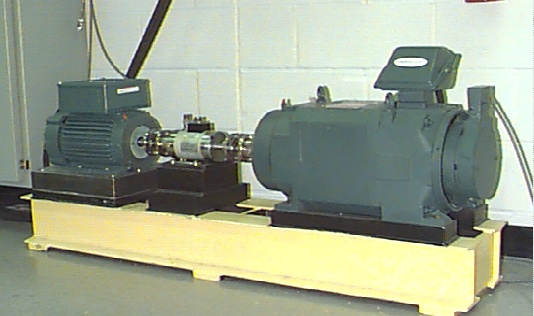
\includegraphics[width=\textwidth,height=0.5\textheight,keepaspectratio]{images/CWRU_teststand}
      \par{\tiny\color{cmuted} CWRU test stand}
    \end{column}
    \begin{column}{0.54\textwidth}
  \begin{block}{Thành phần chính}
    \begin{itemize}
      \item Động cơ điện 2 HP làm nguồn dẫn động, dải tốc độ \textasciitilde{}1720--1797 RPM.
      \item Ổ lăn thử \textbf{SKF 6205-2RS} đặt ở phía dẫn động (Drive End - DE).
      \item Tải 0--3 HP tác động thông qua máy phát hấp thụ lực (Dynamometer).
      \item Lỗi nhân tạo EDM với các đường kính khuyết tật 7, 14, 21 mils.
    \end{itemize}
  \end{block}
  \begin{block}{3 vị trí cảm biến rung}
  \end{block}
    \end{column}
  \end{columns}
  \note{Vì sao cả thế giới dùng bộ dữ liệu này? Vì nó \textbf{có kiểm soát}: người ta gia công vết lỗi với kích thước biết trước, đặt gia tốc kế ngay trên gối đỡ phía dẫn động, đo ở nhiều mức tải.Hãy để ý vị trí cảm biến: nó nằm \textit{trên đường truyền rung} từ ổ tới vỏ máy. Đặt sai chỗ thì tín hiệu lỗi bị chặn, mọi thuật toán phía sau sẽ không thể nhận diện được. Bài học cho nhà máy: cảm biến tốt và đặt đúng chỗ quan trọng hơn một mô hình xịn.\textbf{Giải thích cho kỹ sư mới:}\\• \textbf{EDM (Electro-Discharge Machining):} Gia công bằng tia lửa điện để tạo vết nứt nhân tạo cực kỳ chính xác.\\• \textbf{Mils:} Đơn vị đo độ dài của Mỹ, bằng 1/1000 inch (1 mil $\approx$ 0.0254 mm). Vết lỗi 7 mils $\approx$ 0.18 mm (nhỏ như sợi tóc), 21 mils $\approx$ 0.53 mm.}
\end{frame}

\begin{frame}{4 trạng thái ổ lăn}
  \slidepill{Phần A · Các lớp lỗi}
  \keyidea{Bốn trạng thái --- Normal, lỗi rãnh trong (IR), rãnh ngoài (OR), viên bi (Ball) --- \textbf{vị trí vết lỗi} quyết định ''chữ ký'' rung.}
  \vspace{2pt}
  \begin{columns}[T]
    \begin{column}{0.44\textwidth}
      \centering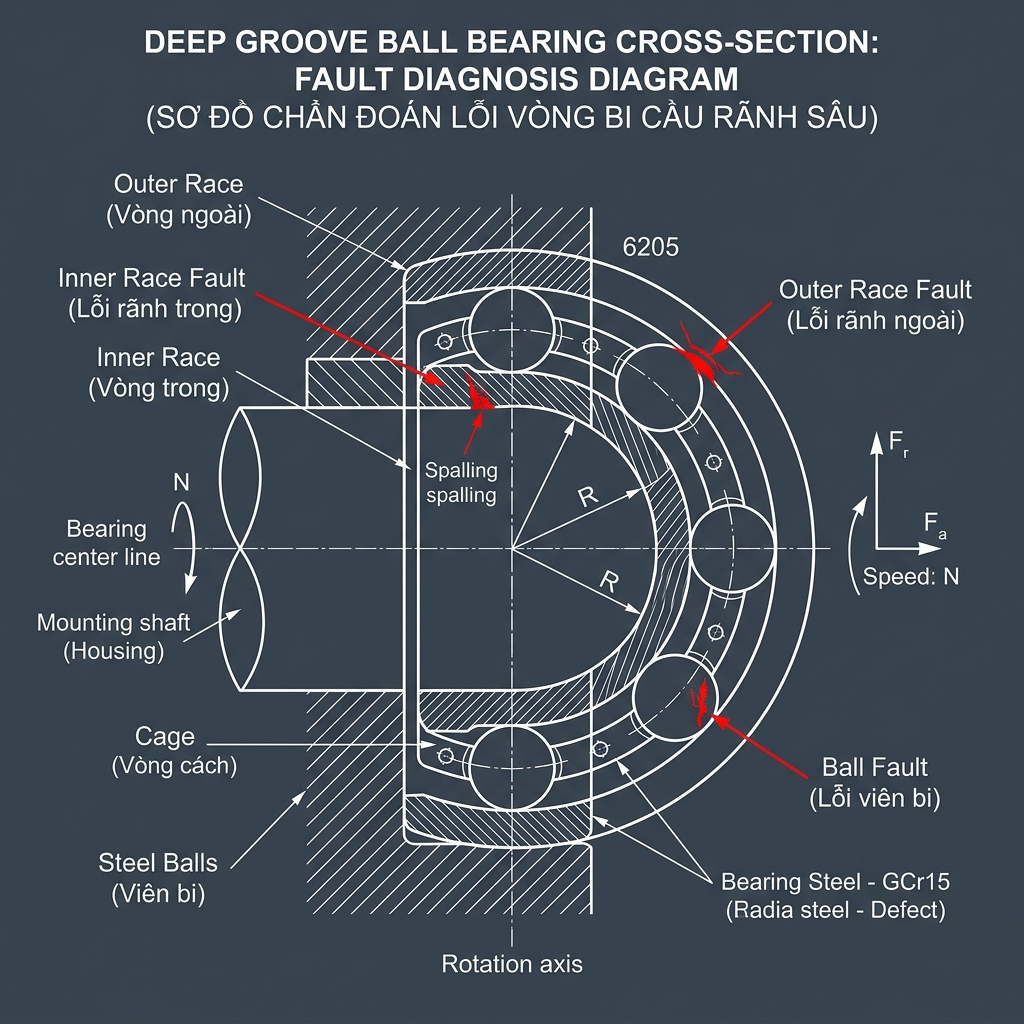
\includegraphics[width=\textwidth,height=0.5\textheight,keepaspectratio]{images/bearing_structure}
      \par{\tiny\color{cmuted} Cấu tạo ổ lăn}
    \end{column}
    \begin{column}{0.54\textwidth}
  \begin{block}{Normal (Bình thường)}
    Không khuyết tật. Sóng rung hình sin nền phẳng lặng, biên độ rất nhỏ, thể hiện trạng thái hoạt động lý tưởng của cơ cấu.\\[2pt]
  \end{block}
  \begin{block}{Outer Race (OR - Lỗi rãnh ngoài)}
    Vết nứt nằm trên rãnh ngoài cố định. Khi bi lăn qua vết nứt tạo ra xung va đập cực mạnh, biên độ lớn và \textbf{chu kỳ lặp lại rất đều đặn}.\\[2pt]
  \end{block}
  \begin{block}{Inner Race (IR - Lỗi rãnh trong)}
    Vết nứt nằm trên rãnh trong quay theo trục. Xung va đập bị \textbf{mô hình điều biên (lên xuống)} do khuyết tật di chuyển ra vào vùng chịu tải.\\[2pt]
  \end{block}
  \begin{block}{Ball (Lỗi viên bi)}
    Vết nứt nằm trên viên bi. Bi vừa tự quay vừa chuyển động quanh trục tạo xung va đập nhỏ, chu kỳ lộn xộn, \textbf{khó phát hiện sớm nhất}.\\[2pt]
  \end{block}
    \end{column}
  \end{columns}
  \warnbox{\textbf{Đánh giá nguy hiểm:} Lỗi rãnh trong (IR) diễn biến nhanh và nguy hiểm nhất do vết nứt chịu ứng suất uốn liên tục. Lỗi viên bi khó bắt nhất vì va chạm xảy ra ở nhiều góc độ tự do.}
  \note{Nhìn hình cấu tạo: rãnh trong quay theo trục, rãnh ngoài đứng yên, đám bi lăn ở giữa. Vết lỗi nằm ở đâu thì cú va xảy ra theo nhịp khác nhau --- đó chính là gốc rễ của BPFI, BPFO, BSF ở slide sau.Một trực giác đáng nhớ: lỗi rãnh ngoài cố định một chỗ $\rightarrow$ cú va \textit{đều như vắt chanh}. Lỗi rãnh trong quay vòng $\rightarrow$ vào vùng chịu tải đập mạnh, ra thì nhẹ $\rightarrow$ biên độ \textit{lên xuống}. Lỗi viên bi loạn nhất, khó thấy nhất. Giữ ba hình ảnh này, lát nữa nhìn dạng sóng các bạn sẽ ''à'' ngay.}
\end{frame}

\begin{frame}{Tần số lấy mẫu \& mức tải}
  \slidepill{Phần A · Điều kiện đo}
  \keyidea{Lấy mẫu 12 kHz (chụp 12.000 điểm rung/giây để bắt xung nhọn); tải tăng $\rightarrow$ vòng quay giảm $\rightarrow$ \textbf{mọi tần số lỗi dịch theo} --- nên mô hình phải đúng bất kể tải.}
  \vspace{2pt}
  \begin{columns}[T]
    \begin{column}{0.46\textwidth}
  \begin{block}{Tần số lấy mẫu (Sampling Rate)}
    Tần số đo đạc \textbf{12 000 Hz} (12 kHz), tức cảm biến gia tốc thu thập chính xác 12.000 giá trị gia tốc (g) trong mỗi giây chạy máy.\\[2pt]
  \end{block}
    \end{column}
    \begin{column}{0.46\textwidth}
  \begin{block}{Hiện tượng Slip (Độ trượt động cơ)}
    Động cơ không đồng bộ xoay chậm lại khi tải tăng:\\[2pt]
  \end{block}
    \end{column}
  \end{columns}
  \warnbox{\textbf{Hệ quả hệ thống (Domain Shift):} Tốc độ động cơ giảm (Slip) làm toàn bộ các tần số lỗi đặc trưng (BPFI, BPFO, BSF) trượt dịch trái xuống. Vì vậy, mô hình AI/ML phải đủ mạnh mẽ để khái quát hóa (generalize) các đặc trưng bất kể sự dịch chuyển tần số do thay đổi tải trọng máy.}
  \goodbox{\textbf{Ý nghĩa:} Tần số lấy mẫu cao là bắt buộc để ''chụp lại'' các xung va đập khuyết tật cực kỳ nhọn và ngắn ngủi (độ rộng cỡ mili giây) ở dải tần số cao trước khi chúng bị suy giảm.}
  \note{Hai con số, nhưng ý nghĩa lớn. 12 000 mẫu mỗi giây nghĩa là ta ''chụp'' được rung tới cỡ vài kHz --- đủ nhanh để thấy cú va nhọn.Quan trọng hơn là bảng tải--tốc độ. Đây là động cơ không đồng bộ: thêm tải thì nó quay chậm lại, 1797 xuống 1730 vòng/phút. Mà tần số lỗi tỉ lệ thẳng với tốc độ quay --- tải đổi thì \textbf{cả bộ tần số lỗi trượt theo}. Hệ quả: mô hình chỉ học ở một mức tải sẽ vấp khi máy chạy tải khác. Nhớ điều này tới phần đánh giá.}
\end{frame}

\begin{frame}{Bearing Defect Frequencies --- SKF 6205}
  \slidepill{Phần A · Tần số đặc trưng lỗi}
  \keyidea{Mỗi loại lỗi có một tần số \textbf{tính được từ hình học ổ lăn} --- đây là ''dấu vân tay'' ta sẽ đi truy tìm.}
  \vspace{2pt}
  \begin{center}
  \begin{tabularx}{\textwidth}{lXXX}
  \toprule
    \textbf{\color{white}Ký hiệu \& Ý nghĩa} & \textbf{\color{white}Công thức cơ bản (ĐATN eq. 2.48--2.51)} & \textbf{\color{white}Hệ số $\times$f$_{r}$} & \textbf{\color{white}@1797 RPM} \\
  \midrule
    \textbf{BPFO}\\Tần số lỗi vòng ngoài & \textit{n}2 · (1 − \textit{d}\textit{D} · cos$\varphi$) · \textit{f}$_{r}$ & 3.585 & \textbf{$\approx$ 107 Hz} \\
    \textbf{BPFI}\\Tần số lỗi vòng trong & \textit{n}2 · (1 + \textit{d}\textit{D} · cos$\varphi$) · \textit{f}$_{r}$ & 5.415 & \textbf{$\approx$ 162 Hz} \\
    \textbf{BSF}\\Tần số bi tự quay & \textit{D}2\textit{d} · [1 − (\textit{d}\textit{D} · cos$\varphi$)$^{2}$] · \textit{f}$_{r}$ & 2.357 & \textbf{$\approx$ 70.6 Hz} \\
    \textbf{FTF}\\Tần số vòng cách & 12 · (1 − \textit{d}\textit{D} · cos$\varphi$) · \textit{f}$_{r}$ & 0.398 & \textbf{$\approx$ 12 Hz} \\
  \bottomrule
  \end{tabularx}
  \end{center}
  \warnbox{\textbf{Tần số \textit{lỗi} bi = 2·BSF $\approx$ 141 Hz:} công thức BSF cho tần số tự quay \textit{cơ bản} (\textasciitilde{}70.6 Hz); nhưng vết lỗi trên bi đập \textbf{cả hai rãnh} mỗi vòng spin $\rightarrow$ xung lỗi bi ở \textbf{2·BSF $\approx$ 141 Hz} (giá trị CWRU lập bảng cho lớp Ball). Công thức chuẩn: ĐATN eq. 2.48--2.51.}
  \note{Các bạn không cần quá lo ngại về các công thức hình học này --- điều cốt lõi cần nhớ là: tần số lỗi không phải phép màu, nó suy ra từ hình học ổ lăn.\\\textbf{Giải thích thuật ngữ:}\\• \textbf{BPFO (Ball Pass Frequency Outer):} Tần số các viên bi lăn qua vết nứt trên vòng ngoài.\\• \textbf{BPFI (Ball Pass Frequency Inner):} Tần số các viên bi lăn qua vết nứt trên vòng trong.\\• \textbf{BSF (Ball Spin Frequency):} Tần số viên bi tự quay quanh trục của nó.\\• \textbf{FTF (Fundamental Train Frequency):} Tần số quay của vòng cách (cage). --- số bi, đường kính bi, góc tiếp xúc --- nhân với tốc độ quay.Ở 1797 vòng/phút: rãnh ngoài \textasciitilde{}107 Hz, rãnh trong \textasciitilde{}162 Hz. Đó là những con số ta sẽ săn trên phổ. Một cái bẫy: lỗi \textit{viên bi} hiện ở 2$\times$BSF $\approx$ 141}
\end{frame}

\begin{frame}{Mỗi lỗi --- một ''dấu vân tay'' tần số}
  \slidepill{Phần A · Bản đồ lỗi thiết bị quay}
  \keyidea{Không chỉ ổ lăn --- mất cân bằng, lệch trục, lỏng, bánh răng đều có dấu tần số riêng; thực tế thường là lỗi \textbf{trộn}.}
  \vspace{2pt}
  \begin{center}
  \begin{tabularx}{\textwidth}{lXX}
  \toprule
    \textbf{\color{white}Loại lỗi} & \textbf{\color{white}Cơ chế lực kích thích} & \textbf{\color{white}Dấu hiệu trên phổ} \\
  \midrule
    \textbf{Mất cân bằng} (unbalance) & Lực ly tâm quay theo trục & Đỉnh trội tại \textbf{1$\times$} (tốc độ quay) \\
    \textbf{Lệch trục} (misalignment) & Mô men uốn tuần hoàn & \textbf{2$\times$}, 3$\times$ (song song); 1$\times$ + dọc trục cao (góc) \\
    \textbf{Lỏng lẻo} (looseness) & Phi tuyến, va đập kết cấu & Nhiều \textbf{bội số điều hòa} 1$\times$,2$\times$,3$\times$… \\
    \textbf{Hỏng ổ lăn} & Chuỗi xung va đập tuần hoàn & \textbf{BPFO/BPFI/BSF} + bội (qua phổ bao) \\
    \textbf{Hỏng bánh răng} & Điều biên lực ăn khớp & Tần số ăn khớp GMF + \textbf{sideband} \\
  \bottomrule
  \end{tabularx}
  \end{center}
  \warnbox{Thực tế nhà máy thường là \textbf{lỗi hỗn hợp} (vd mất cân bằng + ổ lăn) $\rightarrow$ phổ chồng chập. Đây là lý do cần kết hợp \textit{nhiều đặc trưng} + ML, không chỉ nhìn 1 đỉnh. (Khung lý thuyết: ĐATN §2.6)}
  \note{Tôi mở rộng bức tranh một chút, vì ngoài nhà máy ổ lăn hiếm khi hỏng một mình. Mỗi cơ chế lực để lại một dấu khác: mất cân bằng kêu ở đúng 1$\times$ tốc độ quay, lệch trục ở 2$\times$--3$\times$, lỏng bu-lông đẻ ra một dãy bội số, bánh răng thì tần số ăn khớp kèm sideband.Đây chính là lý do ta cần \textbf{machine learning}, không chỉ nhìn một đỉnh phổ: thực tế các dấu này chồng lên nhau, mắt người đọc một phổ rối là chịu. Nhiều đặc trưng cộng với mô hình mới gỡ được mớ bòng bong đó.}
\end{frame}

\begin{frame}[plain]
  \begin{center}
    \vfill
    \textcolor{caccent}{\small\textsc{Tutorial 01}}\\[6pt]
    {\Huge\bfseries\color{white} Khám phá tín hiệu thô}\\[8pt]
    \textcolor{caccent}{\rule{4cm}{1.5pt}}\\[8pt]
    {\small\color{cmuted} Đọc hiểu dạng sóng rung (waveform) thời gian thực của 4 trạng thái vận hành như một kỹ sư chẩn đoán giàu kinh nghiệm.}
    \vfill
  \end{center}
  \note{Bây giờ ta xắn tay vào tín hiệu thật. Tôi muốn các bạn học cách \textit{nhìn} một dạng sóng như một kỹ sư chẩn đoán --- chưa cần toán, chỉ cần con mắt.Đây là bước đầu của một thói quen tốt: luôn nhìn dữ liệu thô trước khi ném vào thuật toán. Nhiều sai lầm đắt giá bắt nguồn từ việc bỏ qua đúng bước này.}
\end{frame}

\begin{frame}{''Chữ ký rung'' 4 trạng thái}
  \slidepill{Tutorial 01 · Waveform}
  \keyidea{Chỉ cần \textbf{nhìn dạng sóng}: Normal phẳng lặng; OR xung đều; IR xung lên--xuống theo vòng quay; Ball thưa, khó thấy.}
  \vspace{2pt}
  \begin{columns}[T]
    \begin{column}{0.44\textwidth}
      \centering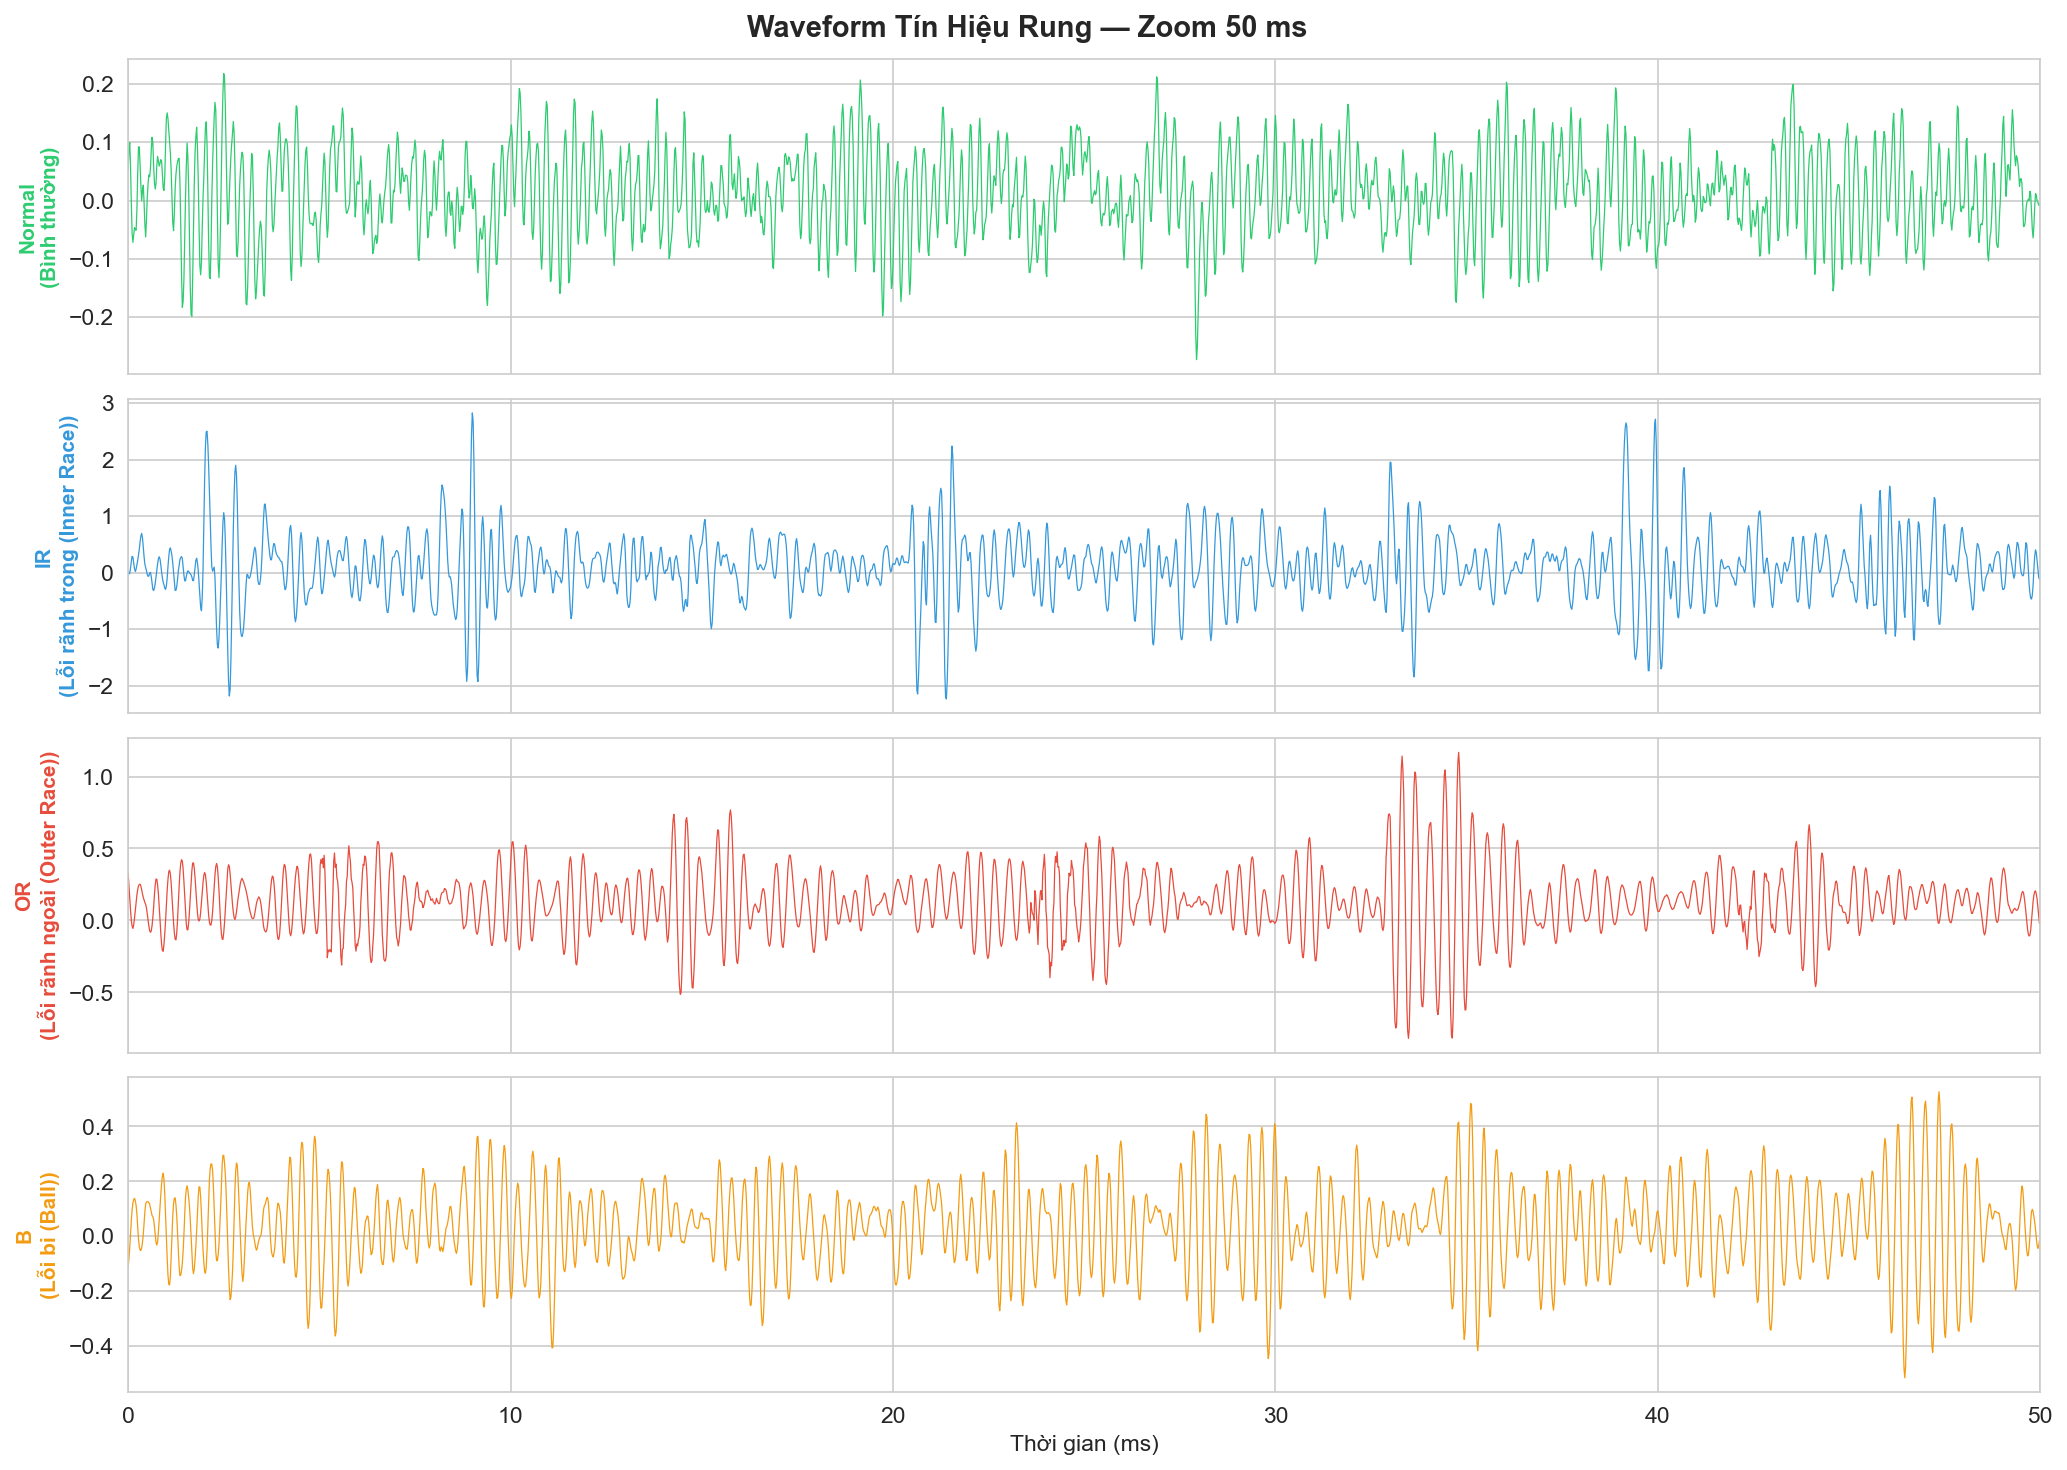
\includegraphics[width=\textwidth,height=0.5\textheight,keepaspectratio]{images/fig_wave}
      \par{\tiny\color{cmuted} Waveform 4 trạng thái (thực tế CWRU)}
    \end{column}
    \begin{column}{0.54\textwidth}
  \begin{block}{Normal}
    Biên độ dao động cực nhỏ (\textless{} 0.2g), sóng phẳng đều và êm dịu, không chứa xung va đập lạ.\\[2pt]
  \end{block}
  \begin{block}{Outer Race (OR)}
    Xuất hiện chuỗi xung nhọn biên độ lớn, lặp lại rất \textbf{tuần hoàn và đều đặn} (do lỗi nằm cố định).\\[2pt]
  \end{block}
  \begin{block}{Inner Race (IR)}
    Các xung nhọn dao động bị \textbf{mô điều biên rõ rệt} (phình to thu nhỏ theo nhịp quay của trục).\\[2pt]
  \end{block}
  \begin{block}{Ball (Lỗi bi)}
    Xung va đập biên độ nhỏ, lưa thưa và phân bố lộn xộn khó định hình (tín hiệu ồn và khó chẩn đoán nhất).\\[2pt]
  \end{block}
    \end{column}
  \end{columns}
  \note{Đây là slide tôi thích nhất, vì nó chứng minh các bạn \textbf{chưa cần thuật toán} cũng đọc được bệnh. Normal: biên độ nhỏ, đều --- thiết bị hoạt động ổn định và êm ái. OR: những cú va đập biên độ lớn và \textit{tuần hoàn rất đều đặn}, vì vết lỗi đứng yên một chỗ.IR: vẫn là xung, nhưng \textit{to nhỏ theo nhịp} --- nhớ slide nãy chứ, vết lỗi quay vào vùng tải rồi lại ra. Ball: lưa thưa, lộn xộn --- ca khó nhất, tôi sẽ nhắc lại suốt khóa. Cái mắt thấy được ở đây chính là cái ta sắp dạy máy \textit{đo} lại bằng con số.}
\end{frame}

\begin{frame}{Định lượng ''mức độ rung''}
  \slidepill{Tutorial 01 · Thống kê}
  \keyidea{Ba con số --- RMS, Peak, Crest factor --- phát hiện \textbf{có} bất thường, nhưng chưa nói được hỏng \textbf{ở đâu}.}
  \vspace{2pt}
  \begin{columns}[T]
    \begin{column}{0.46\textwidth}
  \begin{block}{Đặc trưng thống kê miền thời gian}
    \begin{itemize}
      \item \textbf{RMS (Trị hiệu dụng):} Đo năng lượng rung tổng thể. Thể hiện mức độ phá hủy chung của thiết bị.
      \item \textbf{Peak (Biên độ đỉnh):} Ghi nhận xung va đập tức thời lớn nhất. Rất nhạy khi có mảnh vỡ kẹt.
      \item \textbf{Crest Factor (Hệ số đỉnh):} Chỉ số nhọn (Đỉnh / RMS). Nhạy nhất ở \textbf{giai đoạn đầu khuyết tật} khi xuất hiện xung nhọn nhưng năng lượng RMS tổng thể chưa kịp tăng lên nhiều.
    \end{itemize}
  \end{block}
    \end{column}
    \begin{column}{0.46\textwidth}
  \begin{block}{}
    \begin{itemize}
      \item \textbf{RMS (Trị hiệu dụng):} Đo năng lượng rung tổng thể. Thể hiện mức độ phá hủy chung của thiết bị.
      \item \textbf{Peak (Biên độ đỉnh):} Ghi nhận xung va đập tức thời lớn nhất. Rất nhạy khi có mảnh vỡ kẹt.
      \item \textbf{Crest Factor (Hệ số đỉnh):} Chỉ số nhọn (Đỉnh / RMS). Nhạy nhất ở \textbf{giai đoạn đầu khuyết tật} khi xuất hiện xung nhọn nhưng năng lượng RMS tổng thể chưa kịp tăng lên nhiều.
    \end{itemize}
  \end{block}
    \end{column}
  \end{columns}
  \goodbox{Phát hiện CÓ bất thường (Detection)
Khi có khuyết tật ổ lăn, RMS, Peak và Crest Factor tăng vọt lên \textbf{gấp 2 đến 5 lần} mức vận hành tiêu chuẩn (baseline). Đây là chỉ báo đỏ bắt buộc phải kiểm tra thiết bị ngay lập tức.}
  \badbox{Hạn chế cốt lõi (Diagnosis)
Các đặc trưng miền thời gian này \textbf{hoàn toàn không có khả năng phân loại vị trí lỗi}. Chúng không thể cho biết thiết bị hỏng ở rãnh trong, rãnh ngoài hay do mòn bi. Muốn chẩn đoán bệnh, bắt buộc phải biến đổi sang \textbf{Miền tần số}.}
  \note{Mắt người không scale lên nghìn file được, nên ta cần con số. RMS là trị hiệu dụng, đo năng lượng rung tổng quát --- máy rung càng mạnh, RMS càng lớn. Peak là biên độ đỉnh lớn nhất của sóng rung. Crest factor (Hệ số đỉnh) bằng Đỉnh/RMS, đo độ nhọn sắc của va đập để phát hiện vết nứt từ rất sớm khi năng lượng tổng (RMS) chưa kịp tăng lên nhiều. Nhưng nhân vật tinh tế là \textit{crest factor} = đỉnh chia RMS: nó bắt được cú xung nhọn \textbf{trước khi} năng lượng tổng kịp tăng --- dấu hiệu rất sớm.Cần thành thật với học viên: mấy con số này hét 'có chuyện rồi!' nhưng \textbf{không} nói được rãnh trong hay rãnh ngoài. Muốn biết \textit{ở đâu}, phải bước sang miền tần số --- chính là Tutorial sau.}
\end{frame}

\begin{frame}[plain]
  \begin{center}
    \vfill
    \textcolor{caccent}{\small\textsc{Tutorial 02}}\\[6pt]
    {\Huge\bfseries\color{white} Phân tích tần số}\\[8pt]
    \textcolor{caccent}{\rule{4cm}{1.5pt}}\\[8pt]
    {\small\color{cmuted} Ứng dụng FFT và phân tích Spectrogram để chuyển đổi tín hiệu từ miền thời gian sang miền tần số, tìm ra chính xác lỗi nằm ở đâu.}
    \vfill
  \end{center}
  \note{Tới đây ta đổi kính nhìn: từ miền thời gian sang miền tần số. Câu hỏi chuyển từ ''có rung không'' sang ''rung ở \textit{tần số nào}'' --- và chính tần số mới chỉ ra hỏng ở đâu.Đây là khúc lý thuyết đẹp nhất khóa. Tôi sẽ đi từ trực giác trước, công thức sau --- đúng tinh thần: hiểu ý rồi mới cần ký hiệu.}
\end{frame}

\begin{frame}{FFT: từ thời gian $\rightarrow$ tần số}
  \slidepill{Tutorial 02 · FFT}
  \keyidea{Mọi tín hiệu là \textbf{tổng các sóng sin}; FFT tách xem có những sóng nào --- nhìn theo thời gian thì rối, theo tần số thì lộ cấu trúc.}
  \vspace{2pt}
  \begin{columns}[T]
    \begin{column}{0.44\textwidth}
      \centering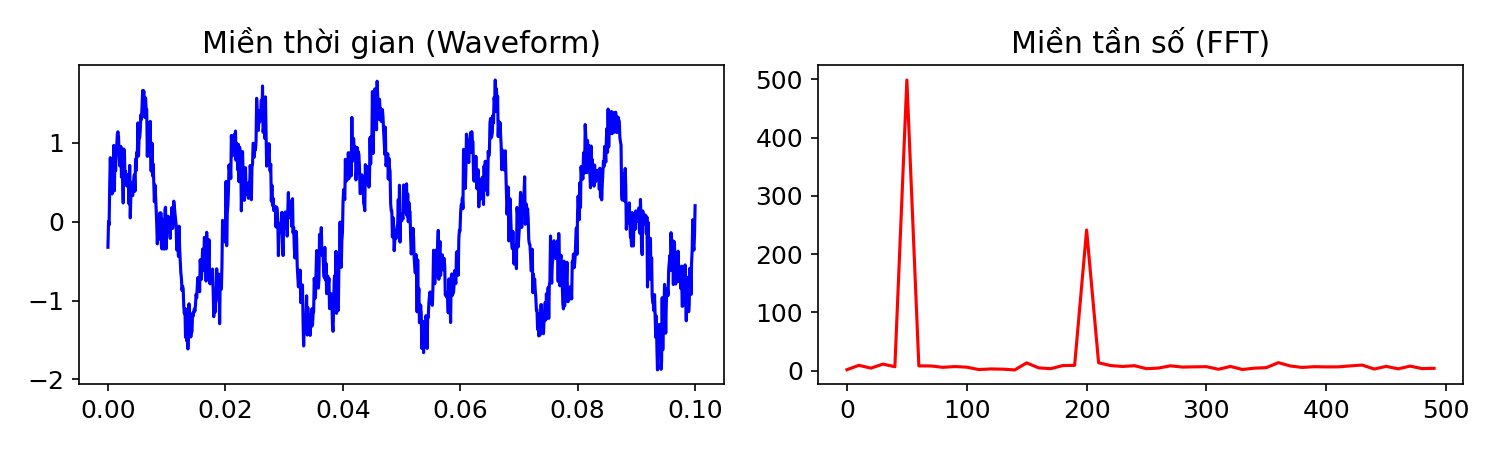
\includegraphics[width=\textwidth,height=0.5\textheight,keepaspectratio]{images/waveform_fft}
      \par{\tiny\color{cmuted} Waveform và FFT}
    \end{column}
    \begin{column}{0.54\textwidth}
  \begin{block}{So sánh hai miền biểu diễn}
  \end{block}
  \formulabox{Biến đổi Fourier rời rạc (DFT / FFT)
\textit{Y}[k] = Σ$_{n = 0..N−1}$ \textit{y}[n] · e$^{−j2$\pi$kn/N}$
Độ phân giải tần số: Δf = f$_{s}$ / N = 12000Hz / 2048 = 5.86 Hz}
  \begin{block}{}
    \textbf{Ví dụ trực giác:} Tai người nghe thấy một hợp âm phức tạp (tín hiệu rung tổng hợp), bộ não tự động tách biệt được các nốt đơn lẻ Đô -- Mi -- Sol. Phép toán FFT thực hiện đúng nhiệm vụ như vậy trên cảm biến rung máy.\\[2pt]
  \end{block}
    \end{column}
  \end{columns}
  \note{Ý tưởng của Fourier, nói một câu: \textbf{mọi tín hiệu đều là tổng của các sóng sin}. FFT hoạt động như một công cụ phân tách tín hiệu thành các sóng sin đơn lẻ, đo lường tần số và biên độ của chúng.Nhìn hai hình: bên trái dạng sóng theo thời gian --- rối mắt; bên phải đúng tín hiệu đó vẽ theo tần số --- từng đỉnh hiện ra. Lần đầu ta thấy \textit{cấu trúc} ẩn dưới sự ồn ào. Nhưng --- tôi để dành cú twist cho slide sau --- với ổ lăn, FFT thô vẫn chưa đủ. Hãy giữ câu hỏi đó trong đầu.}
\end{frame}

\begin{frame}{Mỗi lỗi một ''tần số chữ ký''}
  \slidepill{Tutorial 02 · Tần số chữ ký}
  \keyidea{Lý thuyết: mỗi lỗi một vạch riêng. Thực tế: FFT \textbf{thô} chỉ thấy ''có bất thường'', không gọi đích danh --- phải dùng \textbf{Envelope}.}
  \vspace{2pt}
  \begin{columns}[T]
    \begin{column}{0.44\textwidth}
      \centering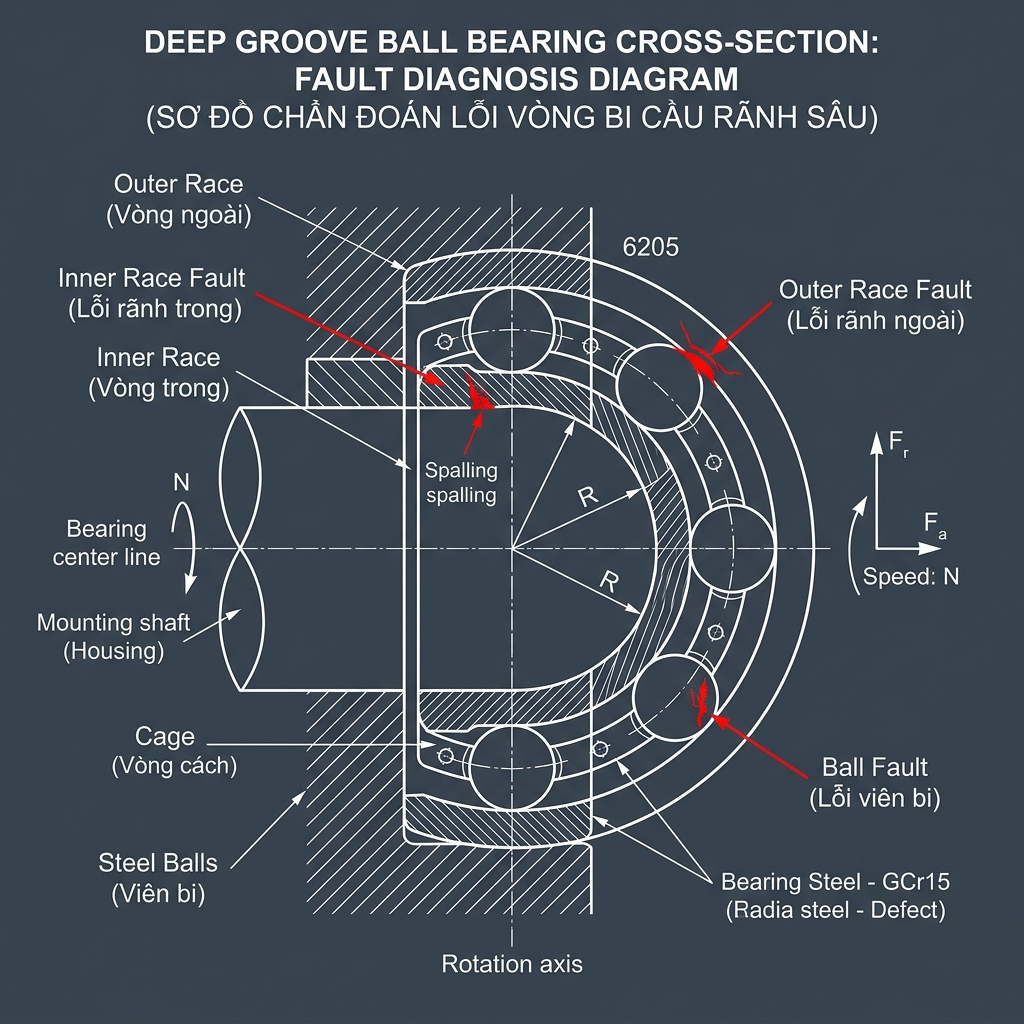
\includegraphics[width=\textwidth,height=0.5\textheight,keepaspectratio]{images/bearing_structure}
      \par{\tiny\color{cmuted} Cấu tạo ổ lăn}
    \end{column}
    \begin{column}{0.54\textwidth}
  \begin{block}{Các tần số khuyết tật lý tưởng (CWRU - 1797 RPM)}
    \begin{itemize}
      \item OR Tần số lỗi rãnh ngoài (BPFO) $\approx$ \textbf{107.4 Hz} + bội số (2x, 3x...)
      \item IR Tần số lỗi rãnh trong (BPFI) $\approx$ \textbf{162.2 Hz} + dải biên (sidebands) $\pm$ \textit{f$_{r}$}
      \item Ball Tần số lỗi viên bi (2•BSF) $\approx$ \textbf{141.2 Hz} (vết nứt đập vào rãnh trong \& ngoài)
    \end{itemize}
  \end{block}
  \begin{block}{Vì sao FFT thô ''MÙ'' với lỗi ổ lăn?}
    Cú va cơ khí của khuyết tật rất ngắn (xung nhọn), gây ra sự kích thích dải tần cực rộng. Trên FFT thô, toàn bộ năng lượng vùng cộng hưởng (vài chục kHz) dâng cao, làm \textbf{chôn vùi vạch lỗi thực sự ở tần số thấp (\textasciitilde{}100 Hz)} khiến ta không thể đọc hoặc định lượng trực tiếp được.\\[2pt]
  \end{block}
  \begin{block}{Phân tích bao (Envelope Analysis) cứu cánh:}
    Bằng cách lọc băng thông (Bandpass) quanh vùng cộng hưởng rộng, sau đó dùng phép biến đổi Hilbert để \textbf{''bóc đường bao''} (giải điều chế) tín hiệu, toàn bộ tần số khuyết tật (BPFO, BPFI) sẽ hiện rõ sừng sững trên phổ bao, cho phép chẩn đoán chính xác.\\[2pt]
  \end{block}
    \end{column}
  \end{columns}
  \note{Đây là điểm tôi muốn các bạn nhớ lâu nhất, nên tôi nói thật chậm. Trên \textit{lý thuyết}, OR cho vạch ở 107 Hz, IR ở 162 Hz --- hoàn hảo như lý thuyết.Trên thực tế, cú va của ổ lăn là một xung rất ngắn, nó kích thích \textbf{toàn dải tần}. Nên FFT thô chỉ cho thấy: nền phổ dâng, vùng cộng hưởng kết cấu (vài kHz) sáng lên --- đủ để nói ''có gì đó sai'', nhưng vạch 107/162 Hz bị \textit{chôn}, không định lượng được. Envelope mới gọi đích danh tần số lỗi. Slide sau tôi chứng minh, bằng vật lý.}
\end{frame}

\begin{frame}{Cộng hưởng \& hệ số Q --- vì sao xung ''khuếch đại''}
  \slidepill{Tutorial 02 · Cộng hưởng \& hệ số Q}
  \keyidea{Cú va dải rộng \textbf{đánh thức tần số cộng hưởng} của kết cấu; cản nhỏ thì đỉnh đó cao \& nhọn (Q lớn) --- chính nó là ''sóng mang''.}
  \vspace{2pt}
  \begin{columns}[T]
    \begin{column}{0.307\textwidth}
  \begin{block}{Hệ dao động 1 bậc tự do (Lò xo - Giảm chấn)}
    Phương trình chuyển động của kết cấu khi chịu xung va đập F(t):\\[2pt]
    Tần số dao động tự nhiên (riêng) ω$_{n}$ và hệ số cản tắt dần ζ:\\[2pt]
    \textbf{Khuếch đại biên độ động (Q-Factor):} Tại tần số cộng hưởng (tần số kích thích bằng tần số riêng, r = ω/ω$_{n}$ = 1): Biên độ khuếch đại tỉ lệ nghịch với cản: \textbf{Q = 1 / (2ζ)}.\\[2pt]
  \end{block}
    \end{column}
    \begin{column}{0.307\textwidth}
  \begin{block}{}
    \textbf{Khuếch đại biên độ động (Q-Factor):} Tại tần số cộng hưởng (tần số kích thích bằng tần số riêng, r = ω/ω$_{n}$ = 1): Biên độ khuếch đại tỉ lệ nghịch với cản: \textbf{Q = 1 / (2ζ)}.\\[2pt]
  \end{block}
    \end{column}
    \begin{column}{0.307\textwidth}
  \begin{block}{Trực giác vật lý: Tiếng chuông ngân}
    Khi gõ nhẹ vào cái chuông, một xung lực cực kỳ ngắn (dải tần rộng) sẽ kích thích và làm chuông ngân vang lâu dài tại đúng tần số riêng cộng hưởng của nó. Kết cấu vỏ máy/gối đỡ ổ lăn tương tự như một chiếc chuông, có tần số riêng dao động (vài kHz).\\[2pt]
  \end{block}
    \end{column}
  \end{columns}
  \goodbox{Vai trò của cộng hưởng kết cấu
Dao động cộng hưởng có hệ số Q lớn sẽ đóng vai trò như một \textbf{sóng mang (carrier frequency f$_{c}$)}, bị điều biến biên độ bởi các cú va đập lặp đi lặp lại của khuyết tật ổ lăn. Phổ bao (Envelope) sẽ lọc quanh dải tần này để bóc tách xung lỗi.}
  \note{Đây là cầu nối lý thuyết, tôi xin một phút ''toán đẹp''. Hình dung gõ vào một cái chuông: bạn gõ một phát \textit{ngắn}, nhưng chuông \textit{ngân dài} ở đúng cao độ riêng của nó. Kết cấu máy cũng có ''cao độ riêng'' --- tần số cộng hưởng ω$_{n}$ = \textbf{√}\textit{k}\textit{m}.Hệ số cản ζ càng nhỏ thì tiếng ngân càng cao và nhọn --- đó là hệ số Q. Mấu chốt: cú va ổ lăn ngắn, dải rộng, nó \textbf{đánh thức} mode cộng hưởng này. Tiếng ''chuông ngân'' đó chính là sóng mang f$_{c}$ --- lát nữa Envelope sẽ lọc đúng quanh nó. Đừng học công thức để nhớ; hãy nhớ \textit{hình ảnh cái chuông}.}
\end{frame}

\begin{frame}{Vì sao FFT thô ''mù'' --- mô hình điều biên}
  \slidepill{Tutorial 02 · Cơ sở lý thuyết}
  \keyidea{Nhịp lỗi không đổi \textbf{cao độ}, nó điều khiển \textbf{biên độ} của tiếng cộng hưởng --- FFT đi tìm cao độ nên ''điếc'' với nhịp.}
  \vspace{2pt}
  \begin{columns}[T]
    \begin{column}{0.307\textwidth}
  \begin{block}{Mô hình toán học điều biên (AM Modulation)}
    \begin{itemize}
      \item \textbf{f$_{c}$ (Tần số mang):} Tần số cộng hưởng kết cấu máy, có năng lượng dao động mạnh nhất (vài kHz).
      \item \textbf{a(t) (Đường bao tức thời):} Dạng sóng chuỗi xung lỗi vật lý tuần hoàn với chu kỳ gõ va chạm T₀ = 1/f$_{defect}$.
    \end{itemize}
  \end{block}
    \end{column}
    \begin{column}{0.307\textwidth}
  \begin{block}{}
    \begin{itemize}
      \item \textbf{f$_{c}$ (Tần số mang):} Tần số cộng hưởng kết cấu máy, có năng lượng dao động mạnh nhất (vài kHz).
      \item \textbf{a(t) (Đường bao tức thời):} Dạng sóng chuỗi xung lỗi vật lý tuần hoàn với chu kỳ gõ va chạm T₀ = 1/f$_{defect}$.
    \end{itemize}
  \end{block}
    \end{column}
    \begin{column}{0.307\textwidth}
  \begin{block}{Thuật toán Hilbert bóc tách vỏ cam}
    Để giải điều chế tín hiệu AM, ta áp dụng phép biến đổi Hilbert \$\textbackslash{}mathcal\{H\}\$ tạo tín hiệu giải tích và lấy trị tuyệt đối để khôi phục đường bao a(t):\\[2pt]
  \end{block}
    \end{column}
  \end{columns}
  \goodbox{\textbf{Hình tượng hóa dễ hiểu:} Tín hiệu rung máy tương tự như \textbf{quả cam}. Xung khuyết tật tần số thấp (múi cam) nằm ẩn bên trong, còn sóng mang tần số cao (vỏ cam) bao bọc bên ngoài. Biến đổi Hilbert chính là quá trình \textbf{''bóc vỏ cam''} để thu về nguyên vẹn các múi cam chứa tần số lỗi BPFO/BPFI/BSF sắc nét.}
  \note{Giờ ghép hai mảnh lại. Mỗi cú va đánh thức tiếng chuông f$_{c}$. Nhưng cú va \textit{lặp theo nhịp lỗi} --- nên tiếng chuông tăng giảm biên độ tuần hoàn đúng theo nhịp BPFO/BPFI. Viết gọn: y(t) = a(t)·cos(2$\pi$f$_{c}$t).f$_{c}$ là cao độ --- FFT nghe thấy. a(t) là cái \textit{bao ngoài} --- nó chứa nhịp lỗi, nhưng không phải một ''cao độ'' nên FFT thô không thấy. Đó là lý do sâu xa FFT thô ''mù'': nó tìm cao độ, mà bệnh nằm ở \textbf{nhịp}. Cách gỡ: Hilbert bóc lấy đường bao a(t), rồi FFT \textit{chính đường bao đó} --- nhịp lỗi hiện ra rõ mồn một.}
\end{frame}

\begin{frame}{4 bước ''bóc'' tần số lỗi --- minh chứng thực tế}
  \slidepill{Tutorial 02 · Envelope Analysis}
  \keyidea{Bốn bước: lọc quanh cộng hưởng $\rightarrow$ Hilbert lấy đường bao $\rightarrow$ FFT đường bao $\rightarrow$ đọc vạch --- và đây là \textbf{minh chứng trên dữ liệu thật}.}
  \vspace{2pt}
  \centering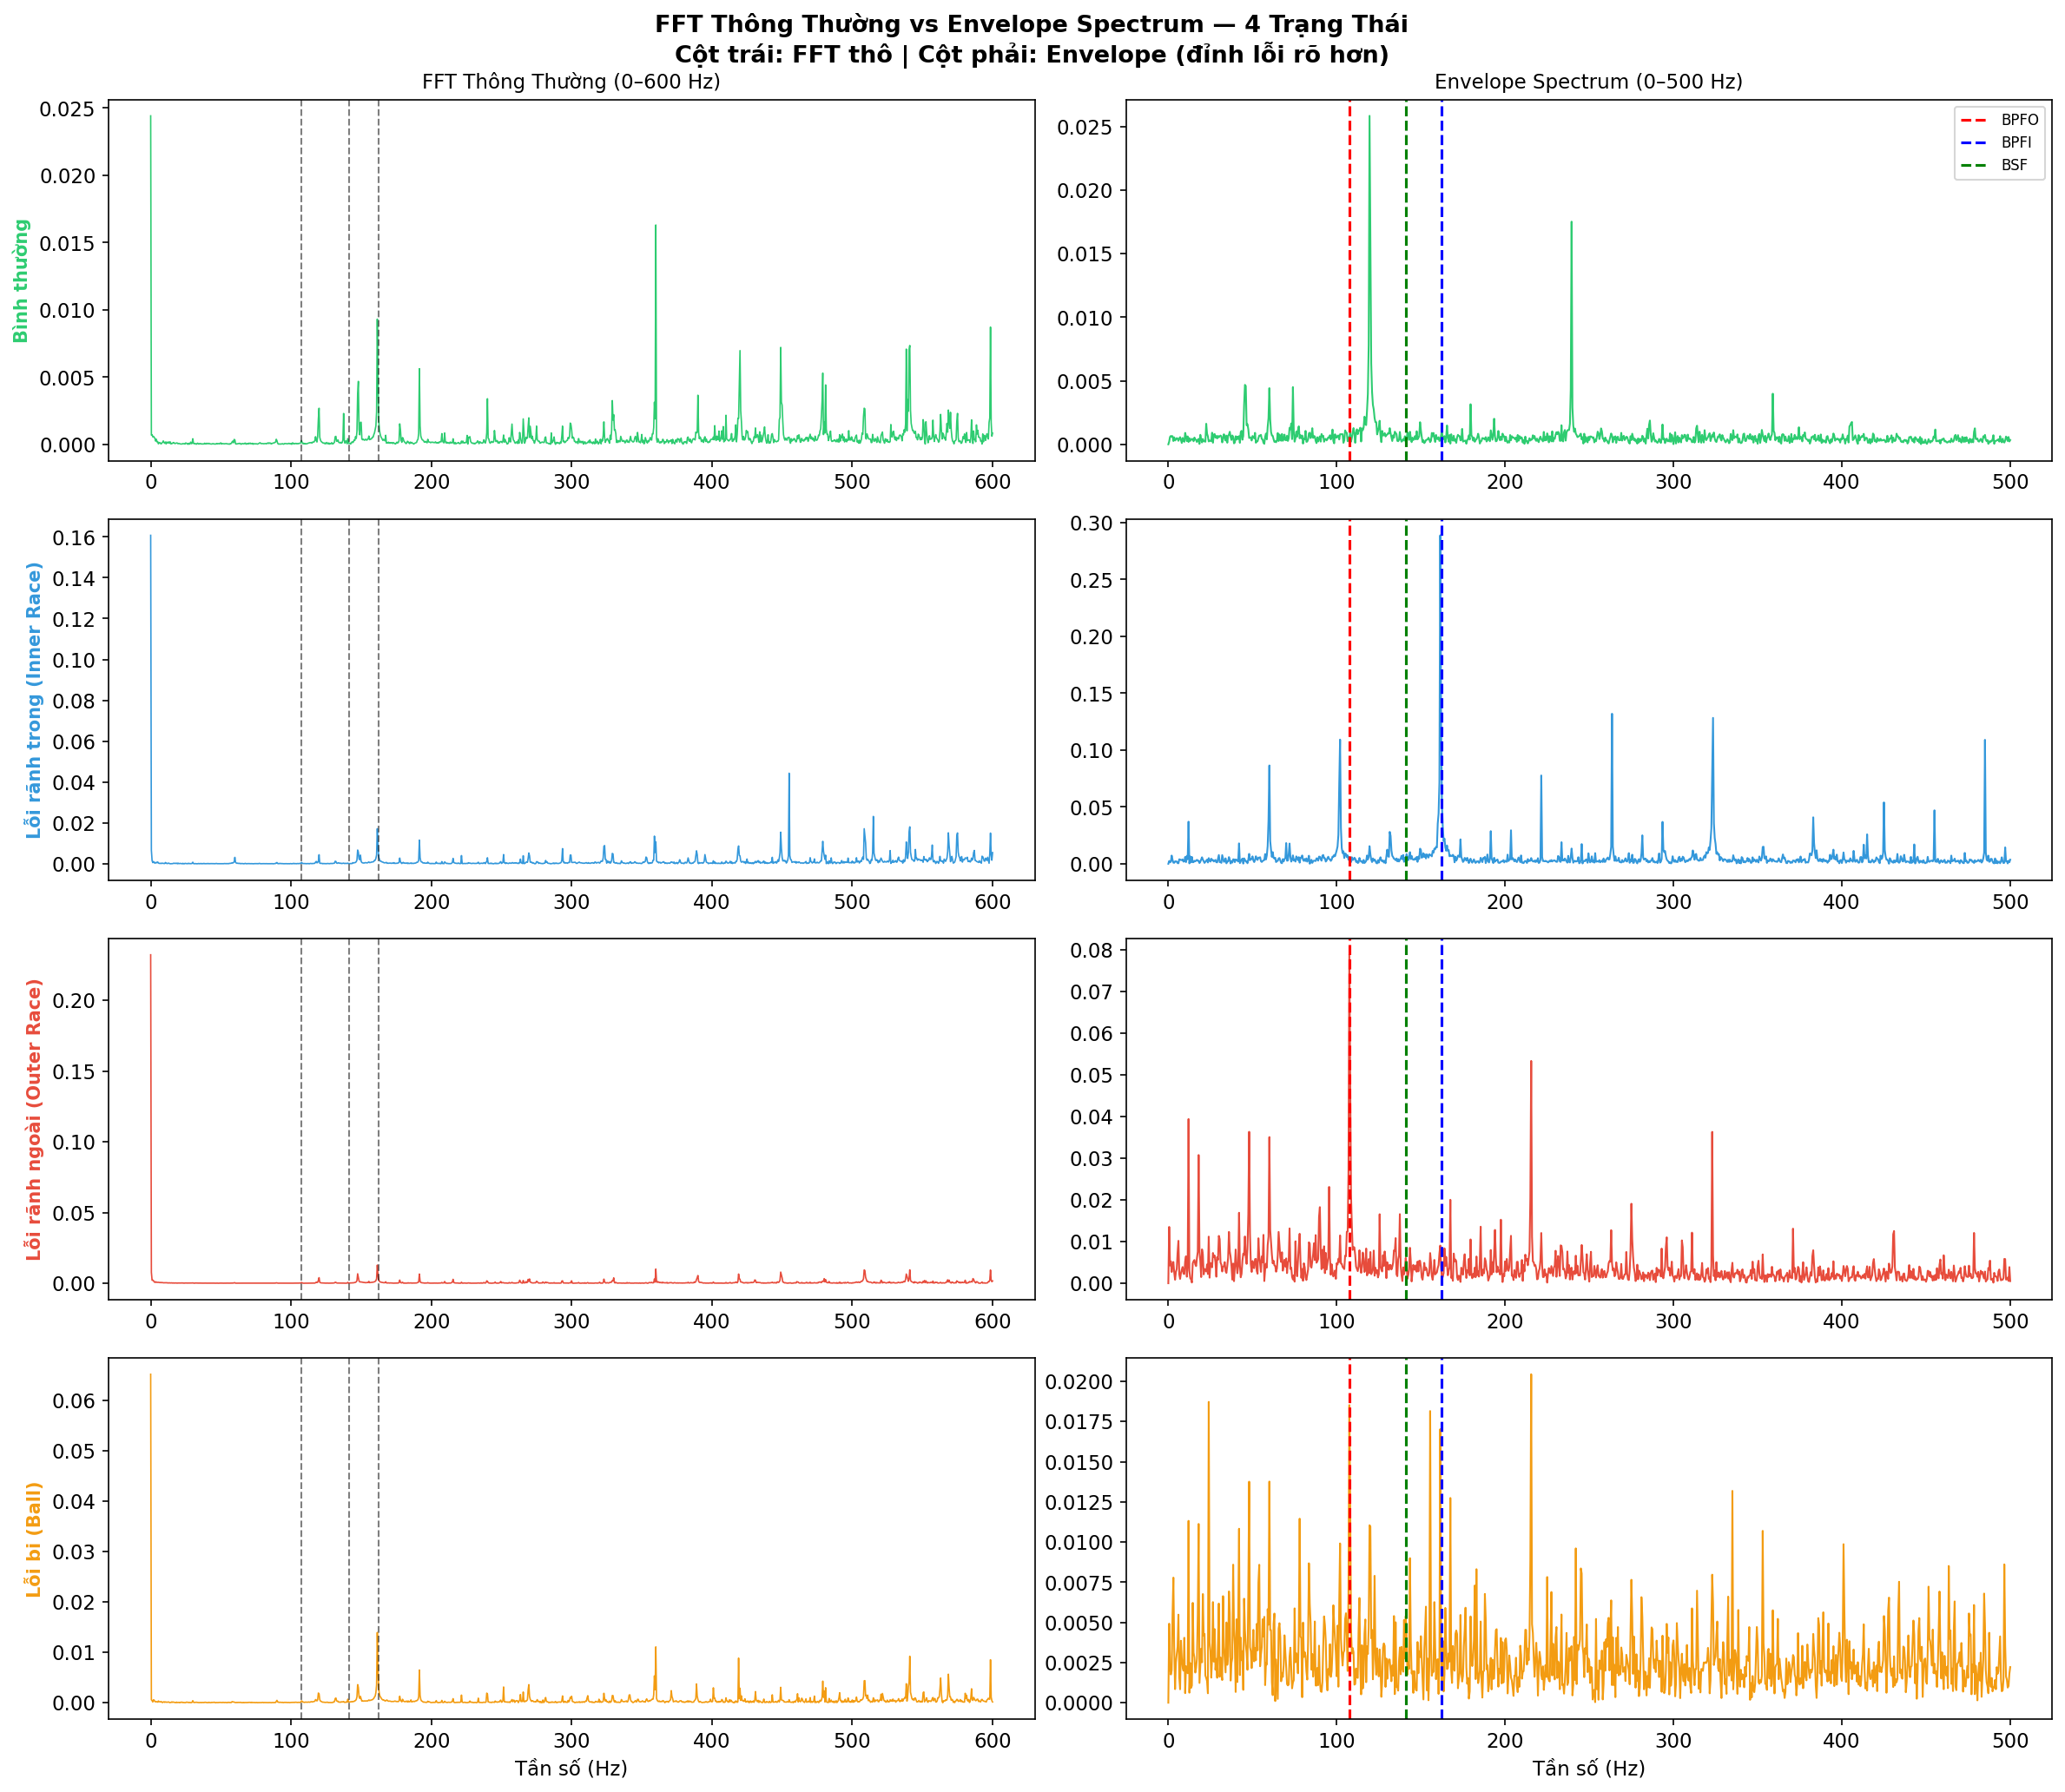
\includegraphics[width=0.9\textwidth,height=0.62\textheight,keepaspectratio]{images/fig_fftenv}
  \par{\tiny\color{cmuted} FFT thô vs Envelope (OR thực tế CWRU)}
  \note{Đây là phần ''thấy mới tin''. Bên trái: FFT thô của một ca OR thật --- gần như vô vọng, chỉ thấy nền dâng. Bên phải: cũng tín hiệu đó qua bốn bước Envelope --- vạch 107 Hz và bội 2$\times$, 3$\times$, 4$\times$ hiện lên \textit{sắc như dao}.Bốn bước, đọc như công thức nấu ăn: lọc băng quanh vùng cộng hưởng để giữ tiếng chuông; Hilbert bóc đường bao; FFT đường bao; đọc đỉnh. Khóa này dùng đặc trưng \textbf{năng lượng dải tần} như cách thay thế gọn cho Envelope đầy đủ --- ý tưởng vật lý y hệt.}
\end{frame}

\begin{frame}{Spectrogram --- bản đồ thời gian $\times$ tần số}
  \slidepill{Tutorial 02 · Spectrogram}
  \keyidea{Spectrogram = \textbf{phim quay chậm của phổ} theo thời gian; xung tuần hoàn hiện thành ''sọc dọc'' sáng lặp đều.}
  \vspace{2pt}
  \begin{columns}[T]
    \begin{column}{0.44\textwidth}
      \centering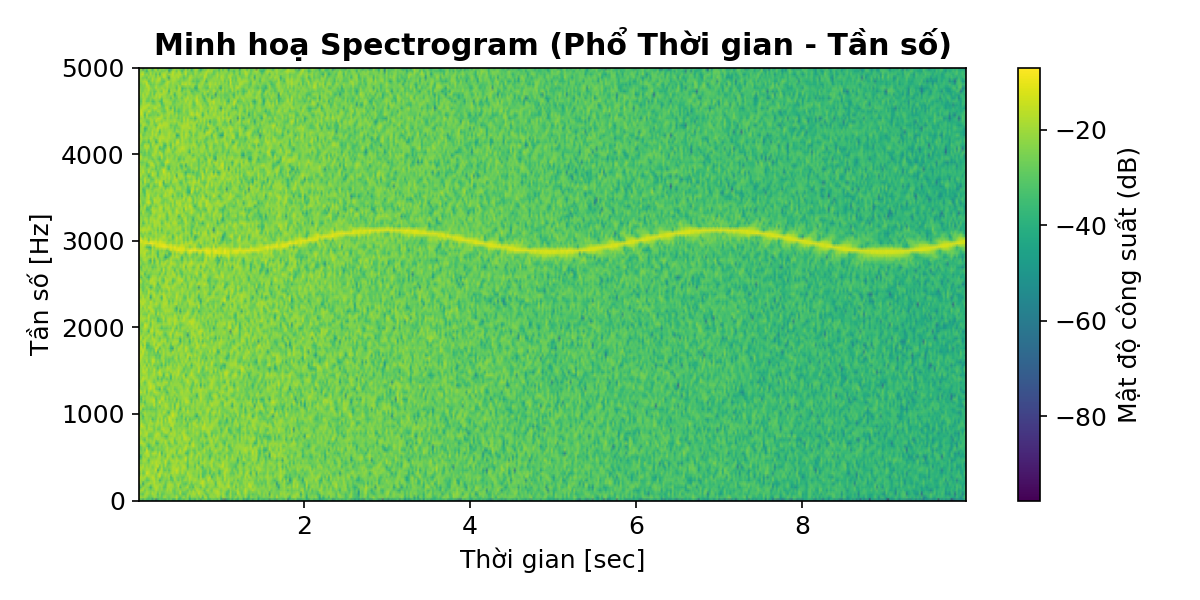
\includegraphics[width=\textwidth,height=0.5\textheight,keepaspectratio]{images/spectrogram_example}
      \par{\tiny\color{cmuted} Spectrogram ví dụ}
    \end{column}
    \begin{column}{0.54\textwidth}
  \begin{block}{Short-Time Fourier Transform (STFT)}
    \begin{itemize}
      \item \textbf{Trục X (Ngang):} Trục thời gian (giây), biểu thị sự biến thiên.
      \item \textbf{Trục Y (Dọc):} Trục tần số (Hz), biểu thị cao độ dao động.
      \item \textbf{Màu sắc:} Thể hiện mật độ năng lượng (màu sáng ấm = năng lượng cao).
    \end{itemize}
  \end{block}
    \end{column}
  \end{columns}
  \goodbox{\textbf{Đọc vị lỗi ổ lăn trên Spectrogram:}\\
          Mỗi cú va khuyết tật cơ khí (xung nhọn dải rộng) xuất hiện cực nhanh và lặp lại tuần hoàn. Trên spectrogram, điều này thể hiện trực quan thành các \textbf{''sọc dọc'' sáng song song cách đều nhau} chạy từ tần số thấp lên tần số cao.
          Lỗi rãnh ngoài OR: Sọc dọc sáng loáng, đều tăm tắp.
Lỗi viên bi Ball: Sọc dọc mờ nhạt, phân bố lộn xộn hơn nhiều.}
  \note{FFT cho một bức ảnh tĩnh --- toàn bộ tín hiệu gộp lại. Nhưng máy thật thay đổi theo thời gian, nên ta cần \textit{cuốn phim}: trục ngang thời gian, trục dọc tần số, màu là năng lượng.Cái mắt cần bắt: nếu lỗi tạo xung tuần hoàn, ta thấy những \textbf{vệt sáng dọc lặp đều} --- chính là nhịp va đập hiện hình. Sọc càng đều càng rõ thì lỗi càng điển hình. Đúng như dự đoán: OR sọc rõ nhất, Ball mờ nhất --- câu chuyện ''Ball khó nhất'' lại quay về.}
\end{frame}

\begin{frame}{Spectrogram 4 trạng thái --- dữ liệu CWRU thật}
  \slidepill{Tutorial 02 · Spectrogram thực tế}
  \keyidea{Trên dữ liệu CWRU thật: OR đậm ''sọc dọc'' nhất, Ball mờ nhất --- \textbf{đúng như lý thuyết tiên đoán}.}
  \vspace{2pt}
  \centering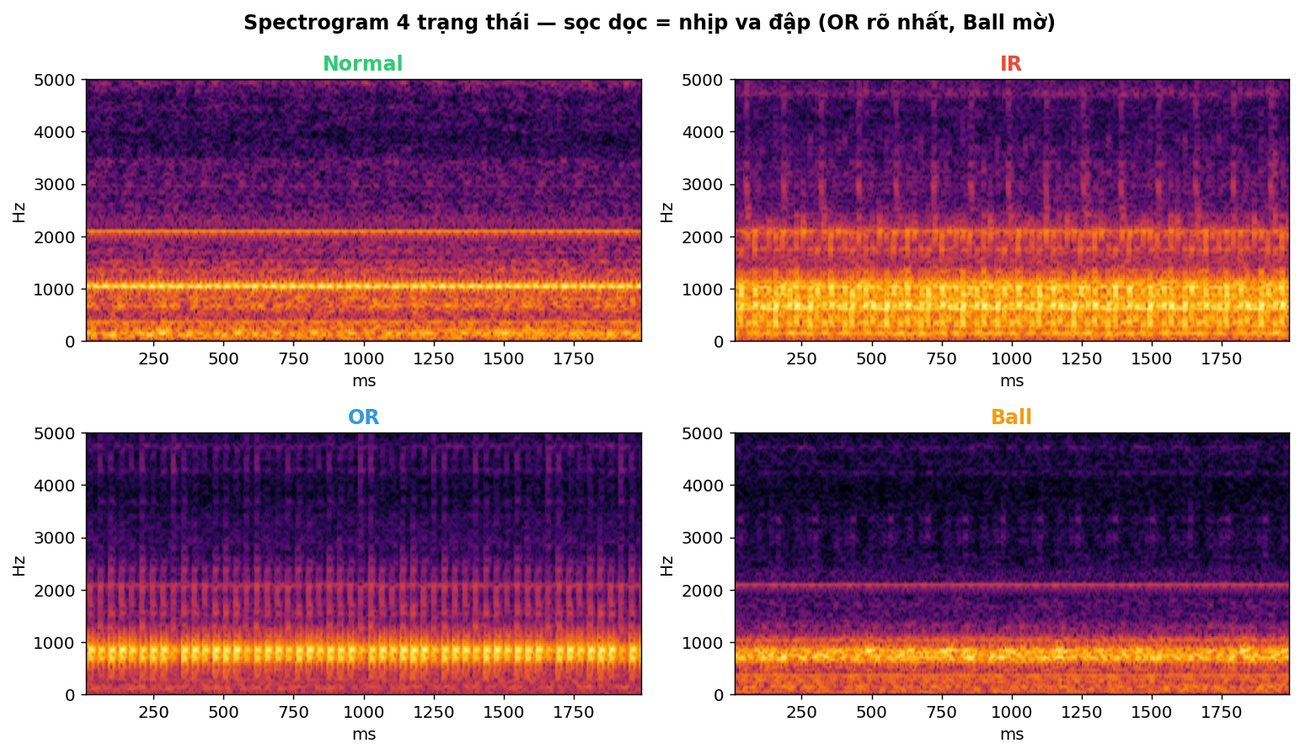
\includegraphics[width=0.9\textwidth,height=0.62\textheight,keepaspectratio]{images/fig_spec}
  \par{\tiny\color{cmuted} Spectrogram 4 lớp CWRU thật}
  \note{Tôi luôn muốn đối chiếu lý thuyết với dữ liệu thật, vì kỹ sư chỉ tin cái nhìn thấy. Đây là spectrogram bốn trạng thái từ chính dữ liệu CWRU.Hãy để mắt tự kết luận: Normal gần như trơn, OR sọc dọc đậm và đều, IR có sọc nhưng nhạt nhịp hơn, Ball lờ mờ --- báo trước mô hình sẽ dễ nhầm Ball nhất. Tới ma trận nhầm lẫn ở Tutorial 04, các bạn sẽ thấy đúng y vậy. Lý thuyết và dữ liệu bắt tay nhau --- đó là lúc ta thật sự \textit{hiểu}.}
\end{frame}

\begin{frame}[plain]
  \begin{center}
    \vfill
    \textcolor{caccent}{\small\textsc{Phần C · Tutorial 03}}\\[6pt]
    {\Huge\bfseries\color{white} Phần C · Trích đặc trưng \& EDA}\\[8pt]
    \textcolor{caccent}{\rule{4cm}{1.5pt}}\\[8pt]
    {\small\color{cmuted} Phương pháp nén dữ liệu sóng thô 2048 chiều thành 19 đặc trưng toán học và thực hiện phân tích EDA trực quan trước khi huấn luyện mô hình.}
    \vfill
  \end{center}
  \note{Ta vừa biết cách \textit{nhìn} và \textit{biến đổi} tín hiệu. Giờ là bước nối với máy học: làm sao biến một đoạn sóng dài thành các đặc trưng có nghĩa mà thuật toán có thể xử lý hiệu quả?Đây là nghệ thuật ''trích đặc trưng'' --- và đi kèm là một cái bẫy rò rỉ dữ liệu mà phần lớn người mới đều mắc. Tôi sẽ chỉ thẳng cái bẫy đó.}
\end{frame}

\begin{frame}{Nén 2048 chiều $\rightarrow$ 19 con số}
  \slidepill{Tutorial 03 · 19 đặc trưng}
  \keyidea{Mỗi đoạn 2048 mẫu nén còn \textbf{19 con số biết nói} --- thống kê thời gian + đặc trưng tần số + năng lượng dải tần.}
  \vspace{2pt}
  \begin{columns}[T]
    \begin{column}{0.44\textwidth}
      \centering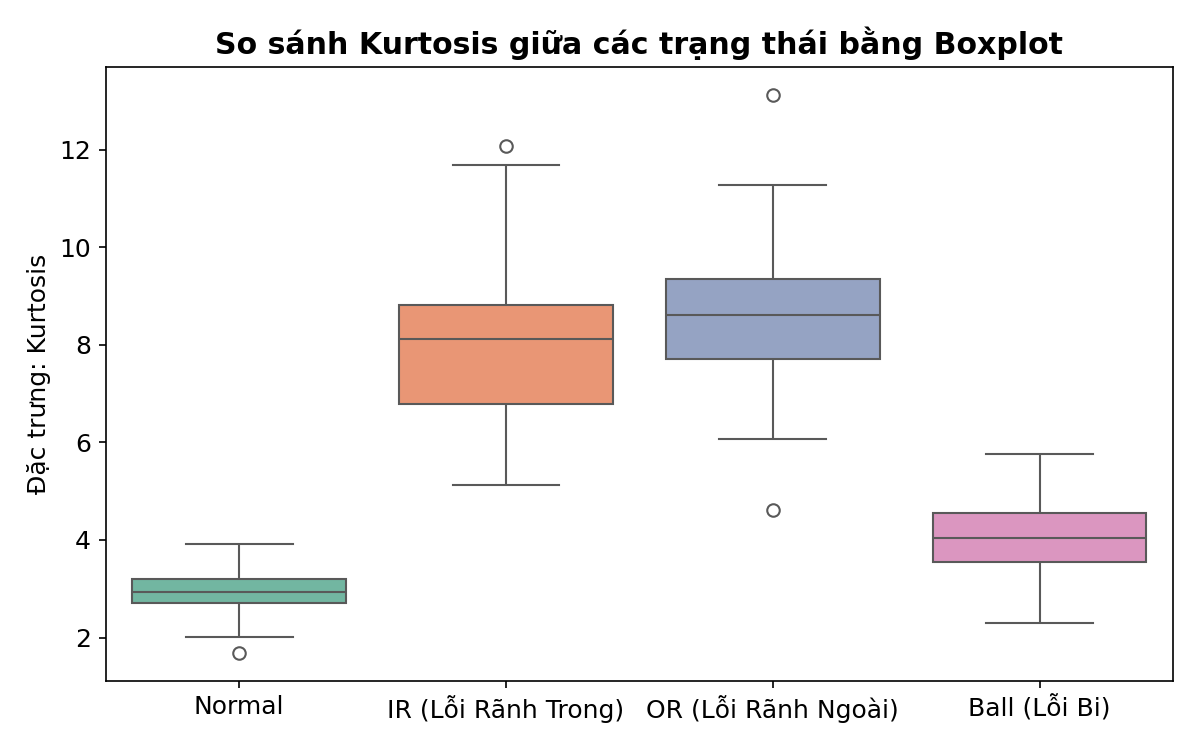
\includegraphics[width=\textwidth,height=0.5\textheight,keepaspectratio]{images/boxplot_example}
      \par{\tiny\color{cmuted} Boxplot đặc trưng theo lớp}
    \end{column}
    \begin{column}{0.54\textwidth}
  \begin{block}{Thời gian (11)}
  \end{block}
  \begin{block}{Tần số (5)}
  \end{block}
  \begin{block}{Dải tần (3)}
  \end{block}
    \end{column}
  \end{columns}
  \warnbox{Tần số lỗi (BPFO 107 · BPFI 162 · lỗi bi 2·BSF 141 Hz) đều trong dải \texttt{0--500 Hz} $\rightarrow$ 1 con số không tách được loại lỗi, nhưng \textbf{kết hợp nhiều đặc trưng} thì ML phân loại tốt.}
  \note{Câu hỏi của slide này: vì sao không đưa trực tiếp 2048 mẫu tín hiệu thô vào mô hình? Vì 2048 con số thô vừa nặng vừa \textit{không có nghĩa} --- mô hình phải tự mò ra cái ta đã biết sẵn từ vật lý.Thay vào đó ta chắt lấy 19 con số \textit{có nghĩa}: rms nói về năng lượng, kurtosis nói về độ nhọn của xung, năng lượng dải tần nói về vùng lỗi. Đây chính là chỗ kiến thức kỹ sư được bơm vào mô hình. Để ý: tần số lỗi 107--162 Hz đều rơi vào dải 0--500 Hz --- một con số đơn lẻ không tách nổi loại lỗi, nhưng nhiều con số ghép lại thì tách được.}
\end{frame}

\begin{frame}{Kurtosis --- ''chuông báo sớm'' (lưu ý định nghĩa!)}
  \slidepill{Tutorial 03 · Kurtosis}
  \keyidea{Kurtosis đo \textbf{độ ''nhọn đuôi''} của phân bố --- xung va đập đẩy nó vọt lên; nhưng phải thống nhất định nghĩa (Pearson, Normal $\approx$ 3).}
  \vspace{2pt}
  \begin{columns}[T]
    \begin{column}{0.46\textwidth}
  \begin{block}{Hai định nghĩa --- rất hay nhầm}
    Code dùng \texttt{kurtosis(x, fisher=False)} $\rightarrow$ Normal $\approx$ \textbf{2.95 $\approx$ 3}, khớp tài liệu.\\[2pt]
  \end{block}
    \end{column}
    \begin{column}{0.46\textwidth}
  \begin{block}{Ngưỡng hành động}
    \begin{itemize}
      \item \textbf{\textgreater{} 3.5} --- theo dõi
      \item \textbf{\textgreater{} 6} --- lên kế hoạch thay
      \item \textbf{\textgreater{} 10} --- hành động ngay
    \end{itemize}
  \end{block}
    \end{column}
  \end{columns}
  \note{Đây là đặc trưng tôi quý nhất, và cũng là cái bẫy định nghĩa kinh điển. Trực giác: máy khỏe thì biên độ rung rải đều như hình chuông Gauss; có vết lỗi thì thỉnh thoảng một cú đập rất mạnh --- \textit{đuôi} phân bố dày lên. Kurtosis đo đúng độ ''dày đuôi'' đó, và nó tăng \textbf{trước cả khi RMS kịp nhúc nhích} --- nên là chuông báo sớm tuyệt vời.\textbf{Giải thích cho người mới:} Kurtosis (Hệ số nhọn) chỉ đơn giản là số đo độ ''nhọn sắc'' của các xung va đập máy. Khi máy chạy êm và khỏe, biên độ rung phân bố đều đặn (Kurtosis $\approx$ 3). Khi bắt đầu xuất hiện vết rỗ hoặc vết nứt nhỏ, các cú va đập nhọn phóng lên làm Kurtosis vọt lên rất cao (ví dụ \textgreater{} 3.5 là cần theo dõi, \textgreater{} 6 là lên lịch thay). Đây là chuông báo sớm nhạy nhất.Nhưng chú ý: scipy mặc định trả Fisher}
\end{frame}

\begin{frame}{Cắt segment \& bẫy rò rỉ dữ liệu}
  \slidepill{Tutorial 03 · Windowing}
  \keyidea{Cửa sổ chồng lấp 50\% cho \textbf{nhiều mẫu hơn} --- nhưng tạo \textbf{bẫy rò rỉ dữ liệu} vô cùng nghiêm trọng nếu chia train/test không đúng phương pháp.}
  \vspace{2pt}
  Cửa sổ \textbf{2048 mẫu} (\textasciitilde{}0.17s, \textasciitilde{}5 vòng quay), trượt \textbf{overlap 50\%} (tăng số mẫu học).\\[2pt]
  \goodbox{$\rightarrow$ Giải pháp: gắn \texttt{file\_id} cho mỗi segment (lưu \texttt{groups.csv}) để Tutorial 04/05 \textbf{chia tập theo file}.}
  \badbox{\textbf{Hệ quả:} hai segment kề nhau dùng chung 1024 mẫu $\rightarrow$ gần như \textit{trùng nhau}. Nếu sau này chia train/test ngẫu nhiên ⇒ ''bản sao'' lọt cả hai bên ⇒ \textbf{accuracy ảo}.}
  \note{Slide này nhỏ nhưng tôi muốn các bạn dừng lại lâu, vì nó là sai lầm đắt nhất cả khóa. Để có nhiều mẫu học, ta trượt cửa sổ chồng lấp 50\% --- hai đoạn cạnh nhau dùng chung \textit{một nửa} dữ liệu, có tính chất gần như tương tự nhau.Giờ tưởng tượng chia train/test ngẫu nhiên: các phân đoạn sóng tương tự nhau bị chia cắt vào cả tập train và test. Mô hình ''học bài rồi thi đúng đề'' --- độ chính xác cao ảo tưởng nhưng không thực tế. Giải pháp: gắn \textbf{file\_id} cho từng đoạn để Tutorial sau chia \textit{theo file}. Chính cái bẫy này kéo accuracy ảo 98\% xuống sự thật \textasciitilde{}78\% --- và 78\% phản ánh đúng năng lực thực chất có giá trị hơn nhiều so với 98\% ảo tưởng.}
\end{frame}

\begin{frame}[plain]
  \begin{center}
    \vfill
    \textcolor{caccent}{\small\textsc{Phần B}}\\[6pt]
    {\Huge\bfseries\color{white} SVM \& Random Forest}\\[8pt]
    \textcolor{caccent}{\rule{4cm}{1.5pt}}\\[8pt]
    {\small\color{cmuted} Nguyên lý hoạt động và so sánh hai thuật toán Machine Learning phân loại chủ lực trong chẩn đoán lỗi thiết bị quay.}
    \vfill
  \end{center}
  \note{Có đặc trưng rồi, giờ mới đến phần mọi người chờ: hai mô hình phân loại chủ lực. Tôi sẽ không nhồi toán.Chỉ cần các bạn nắm \textit{trực giác hình học} của SVM và \textit{trực giác đám đông} của Random Forest. Hiểu ý tưởng thì công thức chỉ còn là xác nhận, không phải rào cản.}
\end{frame}

\begin{frame}{SVM --- ''đường biên an toàn nhất''}
  \slidepill{Phần B · SVM}
  \keyidea{SVM tìm \textbf{đường biên có lề rộng nhất} giữa các lớp; kernel RBF ''nâng chiều'' để tách được cả dữ liệu cong.}
  \vspace{2pt}
  \begin{columns}[T]
    \begin{column}{0.48\textwidth}
      \centering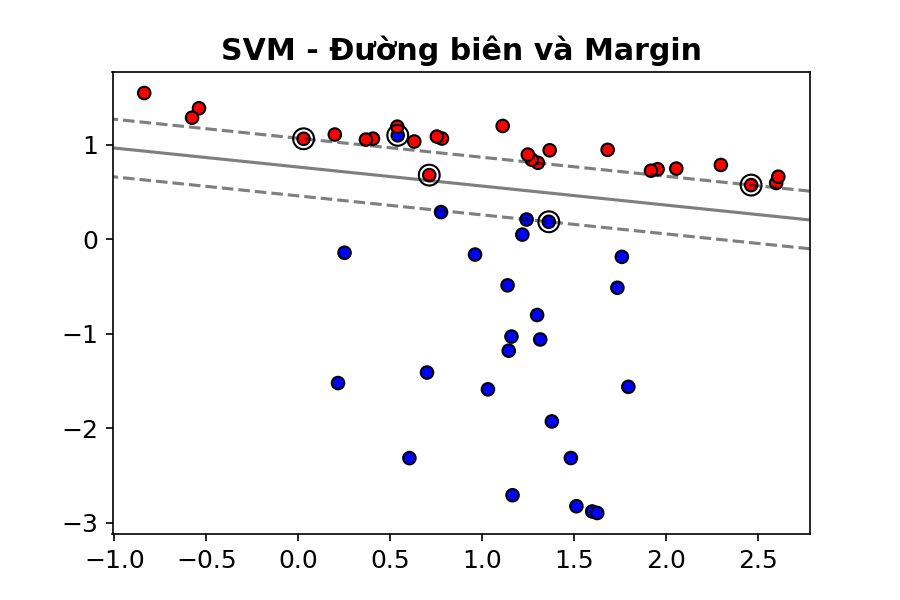
\includegraphics[width=\textwidth,height=0.52\textheight,keepaspectratio]{images/svm_margin}
      \par{\tiny\color{cmuted} SVM margin}
    \end{column}
    \begin{column}{0.48\textwidth}
      \centering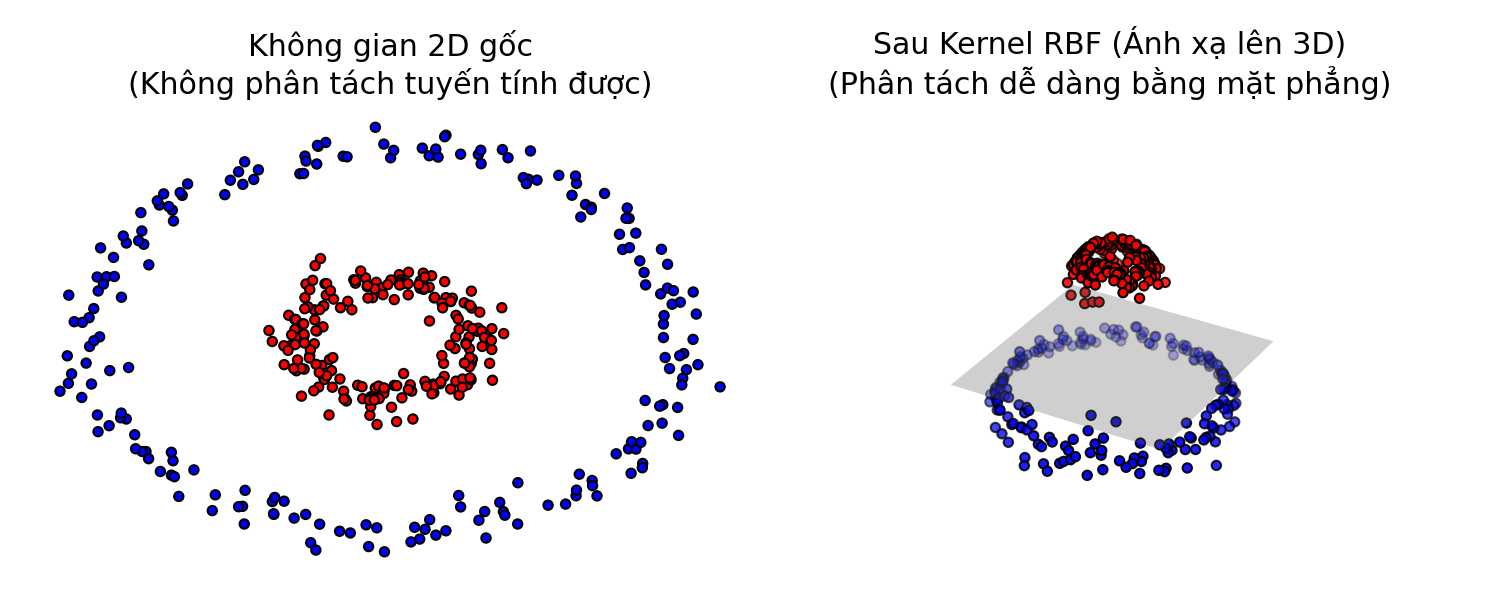
\includegraphics[width=\textwidth,height=0.52\textheight,keepaspectratio]{images/kernel_trick}
      \par{\tiny\color{cmuted} Kernel trick}
    \end{column}
  \end{columns}
  \warnbox{SHAP/predict\_proba cần \texttt{SVC(probability=True)} $\rightarrow$ train chậm \textasciitilde{}3--5$\times$ (Platt scaling).}
  \note{Ý tưởng SVM đẹp một cách hình học. Có hai nhóm điểm, vô số đường tách được --- SVM chọn đường \textit{cách xa cả hai bên nhất}, như con đường có lề an toàn rộng nhất. Lề rộng thì gặp điểm mới ít sai.Dữ liệu cuộn vào nhau không kẻ thẳng được? Kernel RBF ''nhấc'' dữ liệu lên chiều cao hơn, ở đó tách phẳng được rồi chiếu xuống thành biên cong. Lưu ý thực dụng: muốn SHAP/xác suất phải bật \textbf{probability=True}, train chậm 3--5$\times$ vì hiệu chỉnh Platt --- biết trước để khỏi tưởng máy treo.}
\end{frame}

\begin{frame}{Random Forest --- ''hội đồng nhiều cây''}
  \slidepill{Phần B · Random Forest}
  \keyidea{Random Forest = \textbf{hội đồng nhiều cây}, mỗi cây nhìn một góc; biểu quyết đa số nên sai số các cây triệt tiêu nhau.}
  \vspace{2pt}
  \begin{columns}[T]
    \begin{column}{0.44\textwidth}
      \centering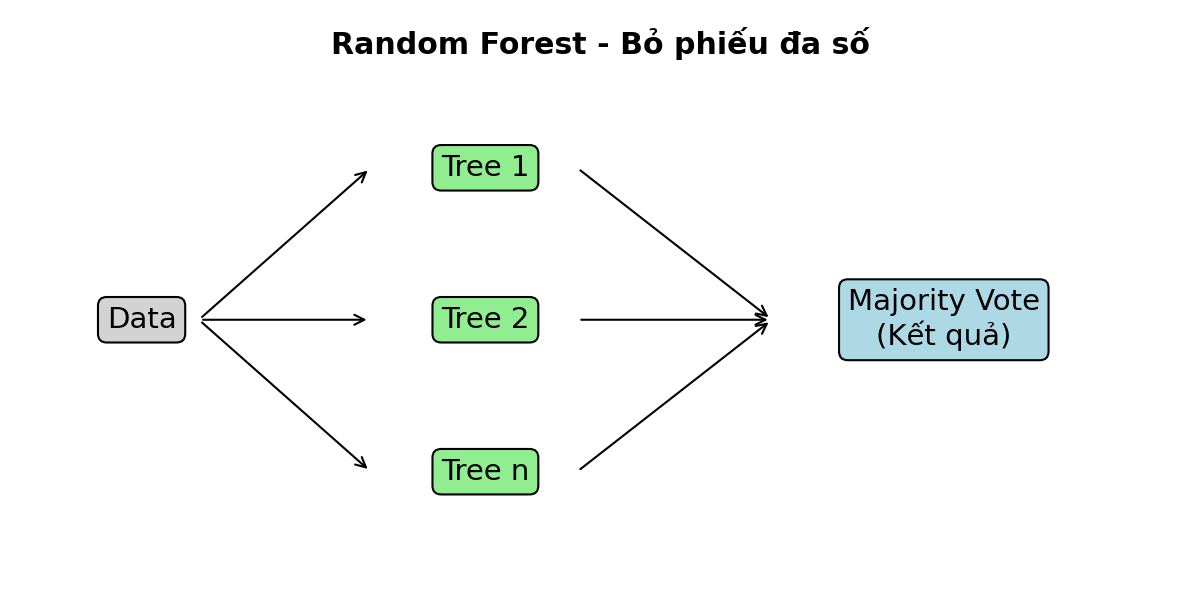
\includegraphics[width=\textwidth,height=0.5\textheight,keepaspectratio]{images/random_forest}
      \par{\tiny\color{cmuted} Random Forest biểu quyết}
    \end{column}
    \begin{column}{0.54\textwidth}
  \formulabox{Cây tách node theo độ thuần Gini · Rừng biểu quyếtGini = 1 − Σ \textit{p}$_{k}$$^{2}$ ; ŷ = mode\{ T$_{1}$(x), …, T$_{B}$(x) \}Mỗi cây: mẫu bootstrap + \textbf{√}\textit{M} đặc trưng ngẫu nhiên $\rightarrow$ sai số các cây triệt tiêu lẫn nhau}
  \begin{block}{Ưu thế cho bài toán này}
    \begin{itemize}
      \item Không cần scale, robust với ngoại lệ
      \item Có \textbf{feature importance} sẵn
      \item \textbf{SHAP TreeExplainer} cực nhanh
    \end{itemize}
  \end{block}
    \end{column}
  \end{columns}
  \goodbox{$\rightarrow$ RF thường là lựa chọn \textbf{triển khai đầu tiên} ở nhà máy.}
  \note{Nếu SVM là một chuyên gia kẻ ranh giới tinh tế, thì Random Forest là một \textit{hội đồng}. Một cây đơn lẻ thì nông và hay học vẹt. Nhưng khi xây dựng một tập hợp gồm hàng trăm cây quyết định độc lập, mỗi cây huấn luyện trên một mẫu bootstrap khác nhau và một nhúm đặc trưng ngẫu nhiên, rồi biểu quyết đa số --- cái sai của cây này bị cái đúng của cây kia bù lại. Đó là sức mạnh ''trí tuệ đám đông''.Với bài toán của ta nó còn ba món quà: không cần chuẩn hóa, có sẵn xếp hạng đặc trưng, và SHAP TreeExplainer chạy cực nhanh. Vì thế ở nhà máy, RF thường là lựa chọn \textit{triển khai đầu tiên}.}
\end{frame}

\begin{frame}{RF chỉ ra đặc trưng nào quan trọng}
  \slidepill{Phần B · Feature Importance}
  \keyidea{RF tự xếp hạng đặc trưng nào quan trọng --- đây chính là \textbf{danh sách nên ưu tiên giám sát online} và đặt ngưỡng cảnh báo.}
  \vspace{2pt}
  \begin{columns}[T]
    \begin{column}{0.44\textwidth}
      \centering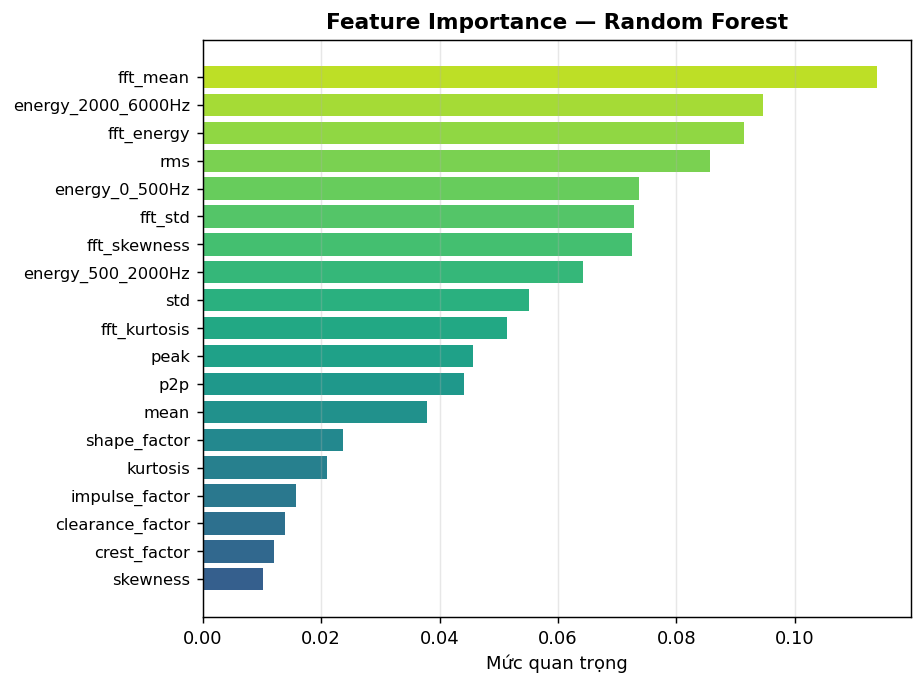
\includegraphics[width=\textwidth,height=0.5\textheight,keepaspectratio]{images/fig_imp}
      \par{\tiny\color{cmuted} Feature importance RF thật}
    \end{column}
    \begin{column}{0.54\textwidth}
  \begin{block}{}
    Các đặc trưng top (năng lượng phổ, rms, fft\_*, kurtosis…) chính là \textbf{chỉ số nên ưu tiên giám sát online} và đặt ngưỡng cảnh báo.\\[2pt]
  \end{block}
  \begin{block}{}
  \end{block}
    \end{column}
  \end{columns}
  \note{Đây là món quà thực dụng của Random Forest cho người vận hành. Nó tự nói: trong 19 đặc trưng, mấy cái này gánh phần lớn quyết định --- thường là năng lượng phổ, rms, đặc trưng FFT, kurtosis.Giá trị thực tế: bạn không cần đo và canh cả 19 chỉ số trên hệ online; hãy ưu tiên vài cái top này, đặt ngưỡng ngay trên chúng. Nhưng nhớ giới hạn: nó chỉ nói mức quan trọng \textit{trung bình toàn cục}. Muốn biết \textit{vì sao một ca cụ thể} được chẩn đoán --- đó là việc của SHAP, Tutorial 05.}
\end{frame}

\begin{frame}[plain]
  \begin{center}
    \vfill
    \textcolor{caccent}{\small\textsc{Tutorial 04}}\\[6pt]
    {\Huge\bfseries\color{white} Huấn luyện \& Đánh giá}\\[8pt]
    \textcolor{caccent}{\rule{4cm}{1.5pt}}\\[8pt]
    {\small\color{cmuted} Thực chiến xây dựng pipeline huấn luyện, tránh bẫy rò rỉ dữ liệu và đánh giá mô hình bằng Confusion Matrix theo góc nhìn hậu quả vận hành.}
    \vfill
  \end{center}
  \note{Phần này tôi xem là \textit{bài học lớn nhất} của cả khóa --- quan trọng hơn cả việc chọn mô hình nào.Đó là: đánh giá cho đúng. Một mô hình 98\% có thể vô dụng, một mô hình 78\% có thể tin được --- nghe nghịch lý, ta sẽ gỡ ngay trong vài slide tới.}
\end{frame}

\begin{frame}{Chia theo FILE, không theo segment}
  \slidepill{Tutorial 04 · Chống rò rỉ}
  \keyidea{Chia tập \textbf{theo file nguồn}, không theo segment --- vì máy mới ngoài đời là \textit{file mới}, mô hình phải được thử đúng như vậy.}
  \vspace{2pt}
  \begin{columns}[T]
    \begin{column}{0.307\textwidth}
  \begin{block}{Chia ngẫu nhiên (Sai)}
  \end{block}
    \end{column}
    \begin{column}{0.307\textwidth}
  \begin{block}{Chia theo file (Đúng)}
  \end{block}
    \end{column}
    \begin{column}{0.307\textwidth}
  \begin{block}{}
  \end{block}
    \end{column}
  \end{columns}
  \note{Quay lại cái bẫy ở slide windowing, giờ ta vá nó. Câu hỏi đúng phải hỏi mô hình là: ''gặp một \textit{cái máy chưa từng thấy}, mày đoán có chuẩn không?''.Nên đơn vị chia phải là \textit{file} --- mọi đoạn từ một file chỉ nằm một bên, train hoặc test, không cả hai. \textbf{GroupShuffleSplit} theo file\_id làm đúng thế, và ta kiểm chứng: 0 file rò rỉ. Đây là khác biệt giữa một con số để khoe và một con số \textit{dám dừng máy theo nó}.}
\end{frame}

\begin{frame}{Độ chính xác: Ảo ảnh rò rỉ và Thực tế khách quan}
  \slidepill{Tutorial 04 · Kết quả thật}
  \keyidea{Chia ẩu cho \textbf{94--98\% (ảo)}; chia theo file cho \textbf{\textasciitilde{}75--79\% (thật)} --- tụt xuống \textasciitilde{}78\% là \textit{tin tốt}, vì giờ con số mới đáng tin.}
  \vspace{2pt}
  \begin{columns}[T]
    \begin{column}{0.46\textwidth}
  \begin{block}{}
    Chia ngẫu nhiên (rò rỉ)\\[2pt]
    94--98\%\\[2pt]
    SVM \textasciitilde{}94\% · RF \textasciitilde{}98\% --- KHÔNG đáng tin\\[2pt]
  \end{block}
    \end{column}
    \begin{column}{0.46\textwidth}
  \begin{block}{}
    Chia theo file (trung thực)\\[2pt]
    \textasciitilde{}75--79\%\\[2pt]
    SVM \textbf{74.6\%} · RF \textbf{\textasciitilde{}78\%} --- thực nghiệm\\[2pt]
  \end{block}
    \end{column}
  \end{columns}
  \goodbox{\textasciitilde{}75--79\%}
  \badbox{94--98\%}
  \note{Đây là slide tôi muốn các bạn nhớ khi rời phòng học. Bên trái: chia ngẫu nhiên đạt 94--98\% --- chỉ là ảo ảnh rò rỉ dữ liệu. Bên phải: chia theo file đạt \textasciitilde{}74--78\% --- phản ánh đúng năng lực thực tế.Phản ứng tự nhiên là tiếc 20\% kia. Nhưng 20\% đó chưa từng có thật --- nó là tiếng vọng của dữ liệu rò rỉ. Thà biết mình đúng 78\% rồi chuẩn bị cho phần sai, còn hơn tin 98\% rồi vỡ mộng khi máy thật hỏng mà mô hình im lặng. Trong kỹ thuật, một con số trung thực luôn quý hơn một con số đẹp.}
\end{frame}

\begin{frame}{Confusion Matrix thực nghiệm (chia theo file)}
  \slidepill{Tutorial 04 · Confusion Matrix thực nghiệm}
  \keyidea{Đừng chỉ nhìn accuracy: soi kỹ ô \textbf{lỗi $\rightarrow$ Normal} --- đó là \textit{bỏ sót}, kiểu sai nguy hiểm nhất.}
  \vspace{2pt}
  \begin{columns}[T]
    \begin{column}{0.44\textwidth}
      \centering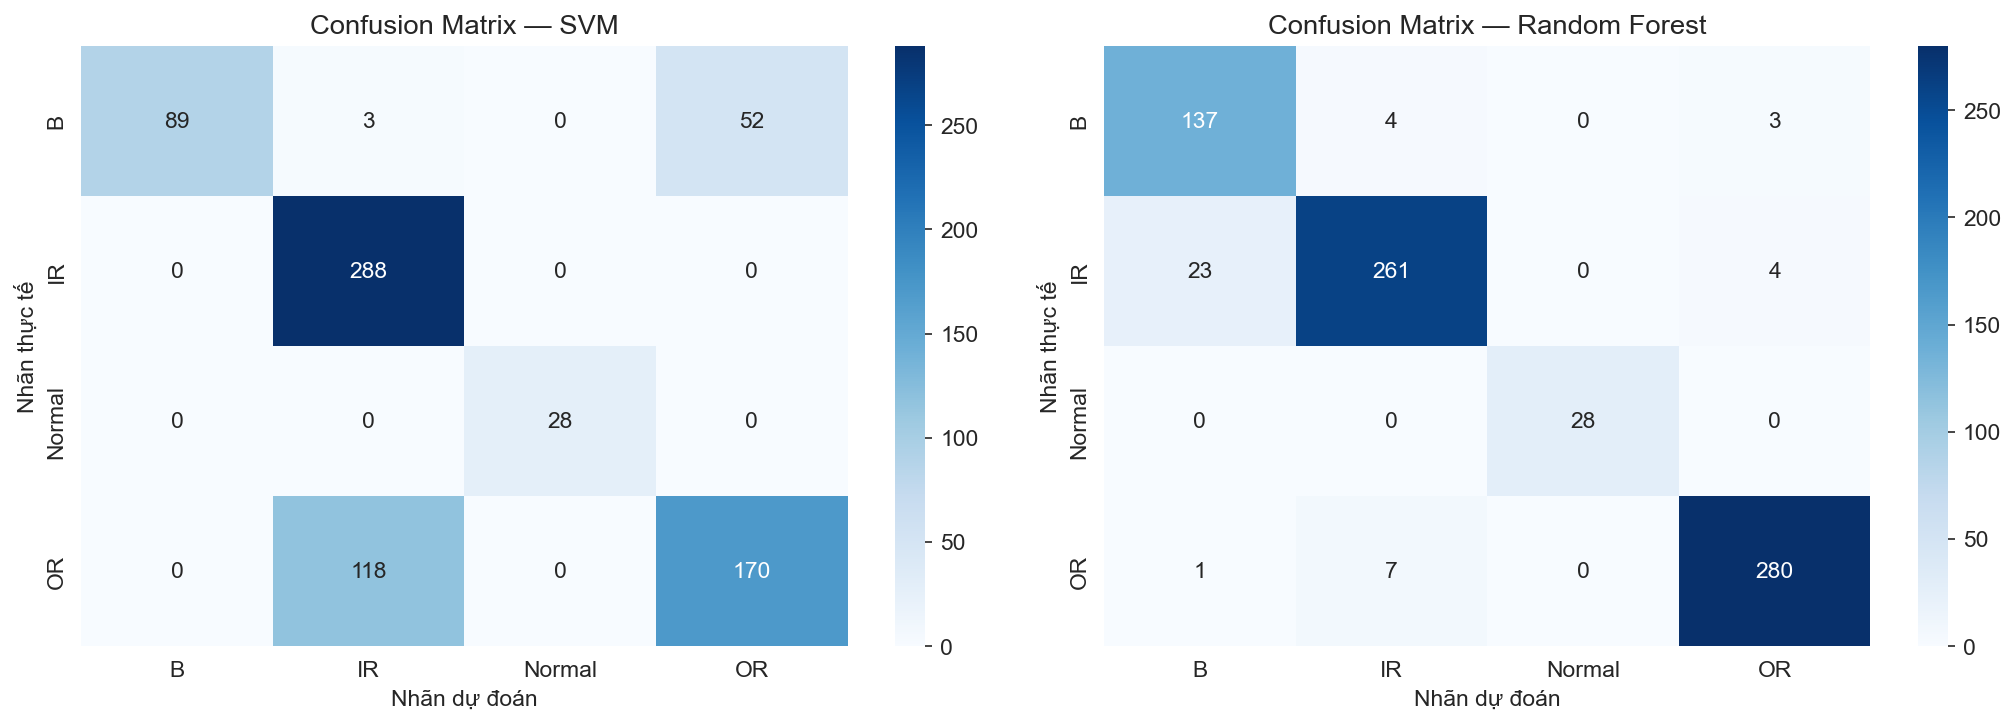
\includegraphics[width=\textwidth,height=0.5\textheight,keepaspectratio]{images/fig_cm}
      \par{\tiny\color{cmuted} Confusion matrix RF thật}
    \end{column}
    \begin{column}{0.54\textwidth}
  \begin{block}{}
    Đường chéo = đúng. Ô ngoài chéo = nhầm. Soi kỹ hàng \textbf{lỗi $\rightarrow$ Normal}: đó là \textit{bỏ sót} --- nguy hiểm nhất.\\[2pt]
  \end{block}
    \end{column}
  \end{columns}
  \badbox{\textasciitilde{}78.6\% (không rò rỉ) thấp hơn nhiều mức ''ảo'' 94--98\%. Đây mới là năng lực thật khi gặp \textbf{file/máy mới}.}
  \note{Accuracy tổng là một con số; ma trận nhầm lẫn mới kể \textit{câu chuyện}. Đường chéo là đoán đúng. Nhưng tôi muốn các bạn dán mắt vào đúng một hàng: lỗi thật mà bị đoán thành Normal.Đó là ca máy đang hỏng nhưng hệ thống nói ''ổn'' --- dẫn thẳng tới dừng máy đột ngột. Một mô hình 78\% mà hiếm khi bỏ sót còn dùng được hơn mô hình 85\% hay bỏ sót. Đây là lúc kỹ sư đọc kết quả bằng \textit{hậu quả}, không bằng con số trung bình.}
\end{frame}

\begin{frame}{Đọc lỗi theo hậu quả}
  \slidepill{Tutorial 04 · Confusion Matrix}
  \keyidea{Đọc lỗi \textbf{theo hậu quả}: bỏ sót (lỗi$\rightarrow$Normal) là đặc biệt nguy hiểm; báo nhầm (Normal$\rightarrow$lỗi) chỉ phát sinh thêm chi phí kiểm tra; nhầm loại thì sai phụ tùng.}
  \vspace{2pt}
  \begin{center}
  \begin{tabularx}{\textwidth}{lXX}
  \toprule
    \textbf{\color{white}Kiểu nhầm} & \textbf{\color{white}Hậu quả} & \textbf{\color{white}Mức} \\
  \midrule
    Lỗi thật $\rightarrow$ đoán \textbf{Normal} (bỏ sót, FN) & Máy hỏng không cảnh báo $\rightarrow$ dừng đột ngột & Rất nguy hiểm \\
    Normal $\rightarrow$ đoán có lỗi (FP) & Kiểm tra thừa, tốn công & An toàn \\
    IR ↔ OR nhầm loại & Chuẩn bị sai phụ tùng & Lưu ý \\
  \bottomrule
  \end{tabularx}
  \end{center}
  \warnbox{Đừng chỉ nhìn accuracy tổng (dữ liệu mất cân bằng: OR rất nhiều, Normal ít) --- soi ô \textbf{''lỗi $\rightarrow$ Normal''}: các ca bỏ sót.}
  \note{Slide này tổng quát hóa thành một bảng để các bạn mang về dùng. Không phải mọi cái sai đều ngang nhau. Lỗi thật $\rightarrow$ Normal: thảm họa, máy gãy không báo. Normal $\rightarrow$ lỗi: chỉ phiền, kiểm tra thừa một lần --- an toàn. IR nhầm OR: không sập máy nhưng chuẩn bị sai phụ tùng, lỡ kế hoạch.Bài học cho người làm bảo trì: khi chỉnh ngưỡng, hãy cố ý lệch về phía ''thà báo nhầm còn hơn bỏ sót'' --- và đừng bao giờ chỉ nhìn accuracy tổng khi dữ liệu lệch lớp.}
\end{frame}

\begin{frame}[plain]
  \begin{center}
    \vfill
    \textcolor{caccent}{\small\textsc{Phần D · Tutorial 05}}\\[6pt]
    {\Huge\bfseries\color{white} SHAP --- Giải thích mô hình}\\[8pt]
    \textcolor{caccent}{\rule{4cm}{1.5pt}}\\[8pt]
    {\small\color{cmuted} Mở nắp ''hộp đen'' thuật toán, ứng dụng lý thuyết trò chơi Shapley để giải thích đóng góp cụ thể của từng đặc trưng vật lý cho mỗi ca chẩn đoán.}
    \vfill
  \end{center}
  \note{Mô hình đoán đúng là chưa đủ --- kỹ sư sẽ hỏi ''dựa vào đâu mày nói thế?''. Không trả lời được thì không ai dám dừng cả dây chuyền.Phần này biến hộp đen thành hộp kính: SHAP. Đây là mảnh ghép biến một mô hình thông minh thành một công cụ \textit{đáng tin để hành động}.}
\end{frame}

\begin{frame}{Shapley value --- ''chia công công bằng''}
  \slidepill{Tutorial 05 · Trực giác}
  \keyidea{Shapley value: chia ''công'' cho từng đặc trưng \textbf{công bằng} bằng cách xét mọi thứ tự ghép nhóm --- ý tưởng từ lý thuyết trò chơi.}
  \vspace{2pt}
  \begin{columns}[T]
    \begin{column}{0.44\textwidth}
      \centering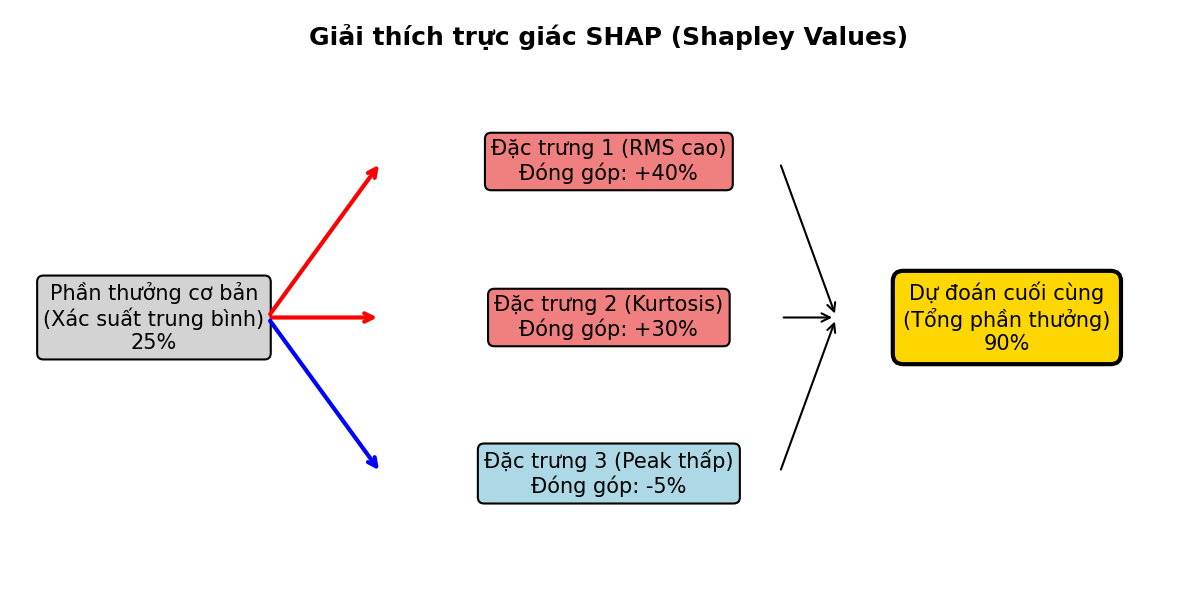
\includegraphics[width=\textwidth,height=0.5\textheight,keepaspectratio]{images/shap_intuition}
      \par{\tiny\color{cmuted} Trực giác Shapley}
    \end{column}
    \begin{column}{0.54\textwidth}
  \begin{block}{}
    3 kỹ sư cùng làm dự án sinh lợi. \textbf{Mỗi người đóng góp bao nhiêu?} $\rightarrow$ xét mọi thứ tự ghép nhóm, lấy trung bình đóng góp biên.\\[2pt]
  \end{block}
  \begin{block}{}
  \end{block}
    \end{column}
  \end{columns}
  \note{Tôi giải thích SHAP không bằng công thức mà bằng một câu chuyện chia thưởng. Ba kỹ sư cùng làm một dự án sinh lời. Mỗi người đáng thưởng bao nhiêu? Cách công bằng: thử mọi thứ tự gia nhập nhóm, xem mỗi người \textit{làm lợi nhuận tăng thêm bao nhiêu} khi bước vào, rồi lấy trung bình. Đó đúng là Shapley value, từ lý thuyết trò chơi 1953.Ánh xạ sang ML: ''kỹ sư'' là đặc trưng, ''lợi nhuận'' là xác suất dự đoán, ''đóng góp'' là SHAP value. Công thức dài kia chỉ nói đúng câu đó. Nhớ: SHAP âm cũng quan trọng --- nó là đặc trưng \textit{phản bác} chẩn đoán, không chỉ cái ủng hộ.}
\end{frame}

\begin{frame}{Summary \& Waterfall}
  \slidepill{Tutorial 05 · Đọc biểu đồ}
  \keyidea{Summary plot = bức tranh toàn cục; Waterfall = \textbf{câu chuyện chẩn đoán cho một ca}, hiện giá trị vật lý để kỹ sư hành động.}
  \vspace{2pt}
  \begin{columns}[T]
    \begin{column}{0.48\textwidth}
      \centering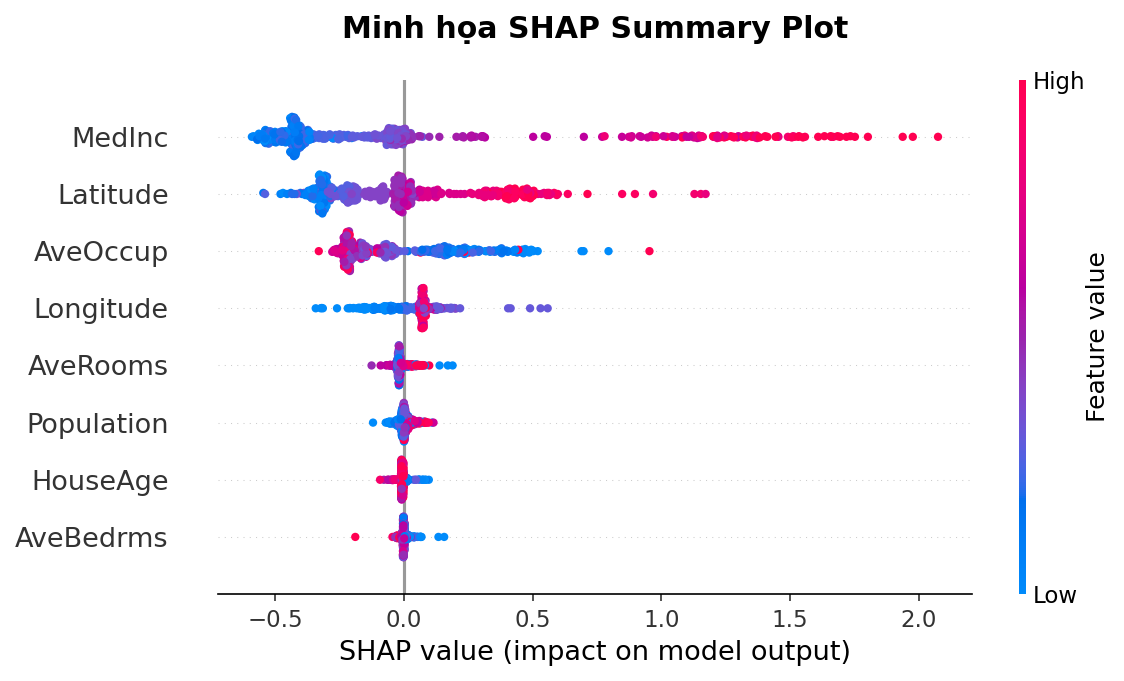
\includegraphics[width=\textwidth,height=0.52\textheight,keepaspectratio]{images/shap_summary}
      \par{\tiny\color{cmuted} SHAP summary plot}
    \end{column}
    \begin{column}{0.48\textwidth}
      \centering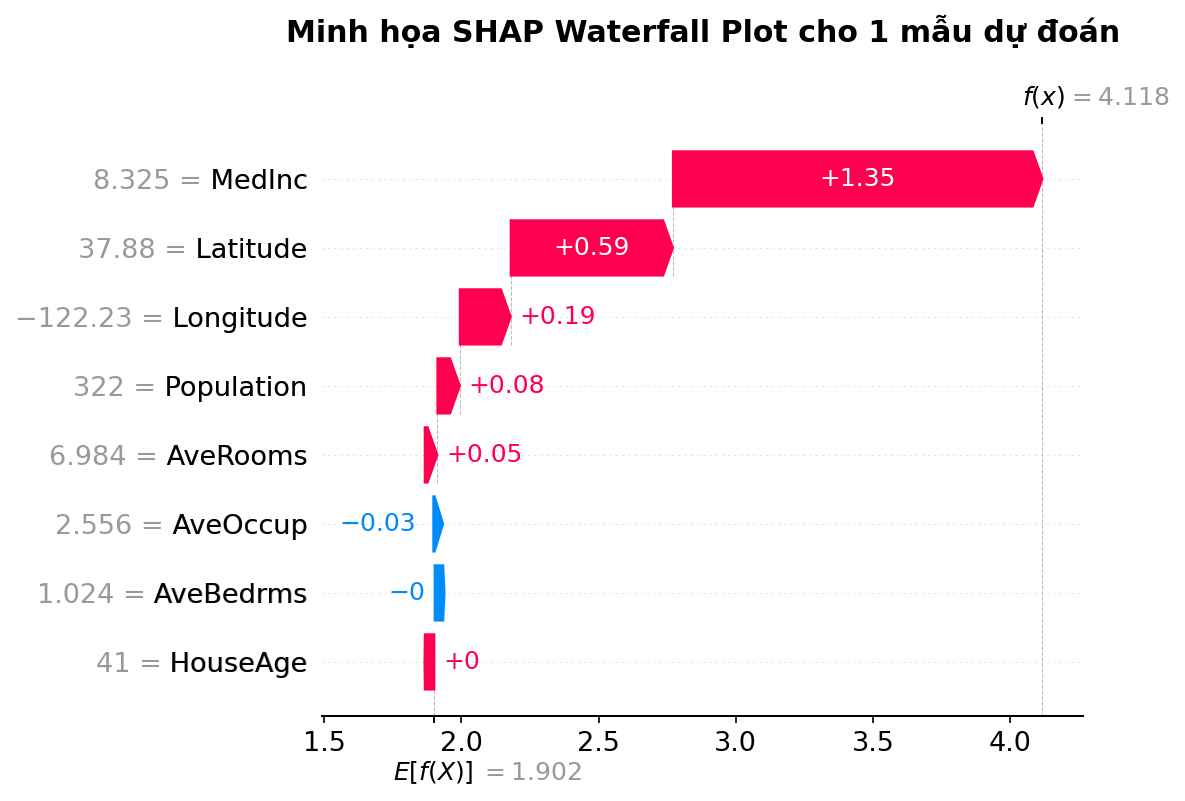
\includegraphics[width=\textwidth,height=0.52\textheight,keepaspectratio]{images/shap_waterfall}
      \par{\tiny\color{cmuted} SHAP waterfall plot}
    \end{column}
  \end{columns}
  \goodbox{Biến waterfall thành \textit{câu chuyện chẩn đoán}: ''kurtosis cao + năng lượng dải lỗi cao $\rightarrow$ chắc chắn OR (xác suất 0.9x)''.}
  \note{Hai biểu đồ, hai câu hỏi. Summary plot: ''nhìn chung mô hình dựa vào gì'' --- tốt để hiểu hệ thống. Waterfall: ''vì sao \textit{ca này} bị gọi là OR'' --- cái kỹ sư cần.Đọc waterfall như một câu chuyện: đỏ là đặc trưng đẩy về phía ''OR'', xanh kéo ngược lại, cộng dồn ra xác suất cuối. Mẹo tôi luôn dùng: hiển thị \textit{giá trị vật lý} chứ không phải giá trị đã chuẩn hóa, để kỹ sư đọc được ''kurtosis = 8, năng lượng dải lỗi cao $\rightarrow$ gần như chắc chắn OR''. Lúc đó AI là một đồng nghiệp biết giải thích.}
\end{frame}

\begin{frame}{Từ SHAP $\rightarrow$ quyết định bảo trì}
  \slidepill{Tutorial 05 · Hành động}
  \keyidea{SHAP không dừng ở ''vì sao'' --- nó \textbf{dẫn thẳng tới hành động bảo trì}: mỗi kiểu chữ ký SHAP ứng một việc cần làm.}
  \vspace{2pt}
  \begin{center}
  \begin{tabularx}{\textwidth}{lXX}
  \toprule
    \textbf{\color{white}SHAP cho thấy} & \textbf{\color{white}Tình trạng} & \textbf{\color{white}Hành động} \\
  \midrule
    rms cao, kurtosis bình thường & Rung tăng, chưa có xung sắc & Bảo dưỡng định kỳ, siết cơ cấu, kiểm tra bôi trơn \\
    \textbf{kurtosis + peak cao} & Vết rỗ/nứt đã hình thành & Lên kế hoạch thay ổ lăn sớm \\
    Năng lượng dải lỗi rất cao & Chẩn đoán tin cậy cao & Chuẩn bị phụ tùng, thay lần dừng máy gần nhất \\
    Đặc trưng ''lạ'' (mean…) quan trọng & Có thể không phải ổ lăn & Kiểm tra lệch trục, mất cân bằng, lỏng bu-lông \\
  \bottomrule
  \end{tabularx}
  \end{center}
  \note{Đây là slide khép vòng tròn của cả khóa: từ một sóng rung, ta đã đi tới \textit{một việc cụ thể để làm sáng mai}. Bảng này đọc như cẩm nang: rms cao nhưng kurtosis bình thường $\rightarrow$ rung tăng chưa có xung sắc $\rightarrow$ bảo dưỡng, siết, kiểm tra bôi trơn. Kurtosis và peak cùng cao $\rightarrow$ vết rỗ đã hình thành $\rightarrow$ lên kế hoạch thay sớm. Năng lượng dải lỗi rất cao $\rightarrow$ chuẩn bị phụ tùng, thay ở lần dừng máy gần nhất.Và nếu mấy đặc trưng ''lạ'' lại quan trọng $\rightarrow$ có khi không phải ổ lăn, đi soi lệch trục hay lỏng bu-lông. SHAP biến chẩn đoán thành quyết định --- đó là toàn bộ lý do ta học nó.}
\end{frame}

\begin{frame}{Accuracy cao $\neq$ dùng được ngay}
  \slidepill{Hạn chế}
  \keyidea{Accuracy cao trên CWRU \textbf{$\neq$ áp dụng được ngay} ngoài nhà máy --- phải hiệu chỉnh trên dữ liệu máy thật trước khi tin.}
  \vspace{2pt}
  \begin{itemize}
    \item \textbf{Domain shift lớn:} CWRU (ổ SKF 6205, EDM, phòng lab) $\neq$ máy nhà máy (ổ khác, lỗi tự nhiên, nhiễu môi trường).
    \item Mô hình 78\% trên CWRU có thể tụt mạnh trên dữ liệu máy thật.
    \item \textbf{Bắt buộc:} thu thập dữ liệu máy thật $\rightarrow$ \textit{calibrate / huấn luyện lại} trước khi tin để dừng máy.
  \end{itemize}
  \warnbox{CWRU là môi trường \textbf{học phương pháp}, không phải mô hình ''áp dụng ăn sẵn'' cho mọi nhà máy.}
  \note{Tôi sẽ thành thật, vì một người thầy tử tế phải nói cả phần khó. Mọi thứ ta vừa làm dựa trên CWRU: một loại ổ SKF 6205, lỗi gia công EDM, phòng lab sạch. Máy của các bạn: ổ khác, lỗi mọc tự nhiên, nhiễu môi trường đầy. Đó là ''domain shift'', và mô hình 78\% trên CWRU hoàn toàn có thể tụt mạnh ngoài đời.Đừng hiểu sai thông điệp khóa học: cái mang về không phải file mô hình này, mà là \textit{phương pháp}. Muốn dùng thật thì bắt buộc thu dữ liệu máy mình, hiệu chỉnh hoặc huấn luyện lại --- rồi mới dám để nó quyết định dừng máy.}
\end{frame}

\begin{frame}{Từ chẩn đoán $\rightarrow$ mức khẩn cấp (ISO 10816/20816)}
  \slidepill{Tiêu chuẩn · Phân cấp mức nghiêm trọng}
  \keyidea{ML cho biết \textit{loại lỗi}; biên độ rung + ISO + \textbf{xu hướng theo thời gian} cho biết \textit{mức khẩn cấp} --- phải kết hợp cả hai.}
  \vspace{2pt}
  \begin{center}
  \begin{tabularx}{\textwidth}{lXX}
  \toprule
    \textbf{\color{white}Vùng} & \textbf{\color{white}Tình trạng} & \textbf{\color{white}Hành động} \\
  \midrule
    \textbf{A} & Máy mới / tốt & Vận hành bình thường \\
    \textbf{B} & Chấp nhận, chạy dài hạn được & Theo dõi định kỳ \\
    \textbf{C} & Cảnh báo --- không nên chạy lâu & Lên kế hoạch bảo trì, tăng tần suất đo \\
    \textbf{D} & Nguy hiểm --- hư hại có thể xảy ra & Dừng máy / can thiệp ngay \\
  \bottomrule
  \end{tabularx}
  \end{center}
  \warnbox{ML cho biết \textit{loại lỗi}; chỉ số rung + ISO + \textbf{xu hướng (trend)} cho biết \textit{mức khẩn cấp}. Kết hợp cả hai mới ra quyết định bảo trì tối ưu. (ĐATN §1.3)}
  \note{Một mảnh ghép cuối nhiều người quên. Mô hình nói ''đây là lỗi OR'' --- tốt, nhưng \textit{nặng tới đâu}? Trả lời câu đó không phải việc của ML mà của tiêu chuẩn rung quốc tế: ISO 10816/20816 chia vùng A xanh tới D đỏ theo biên độ rung.Quan trọng không kém là \textit{xu hướng}: một giá trị tĩnh ít nói, nhưng đường đi lên dốc theo tuần thì hét lên ''sắp hỏng''. Công thức quyết định cuối: ML cho \textit{loại lỗi}, ISO cho \textit{mức nghiêm trọng}, trend cho \textit{còn bao lâu}. Gộp ba thứ mới ra lịch bảo trì tối ưu.}
\end{frame}

\begin{frame}{Key Takeaways}
  \slidepill{Tổng kết}
  \keyidea{Nếu chỉ nhớ một điều: \textbf{chia theo file} để có sự thật, và \textbf{dùng vật lý + SHAP} để con người dám hành động theo AI.}
  \vspace{2pt}
  \begin{columns}[T]
    \begin{column}{0.46\textwidth}
  \begin{block}{Kỹ thuật}
    \begin{itemize}
      \item Chữ ký @1797 RPM: BPFO 107 / BPFI 162 / lỗi bi 2·BSF 141 Hz
      \item Kurtosis Pearson (Normal$\approx$3) --- chuông báo sớm
      \item Envelope \textgreater{} FFT thô cho lỗi ổ lăn
    \end{itemize}
  \end{block}
    \end{column}
    \begin{column}{0.46\textwidth}
  \begin{block}{Phương pháp}
    \begin{itemize}
      \item \textbf{Chia theo file} --- không thì accuracy ảo
      \item RF + SHAP: nhanh, giải thích được
      \item Hiển thị giá trị vật lý để kỹ sư hành động
      \item Calibrate trên máy thật trước khi triển khai
    \end{itemize}
  \end{block}
    \end{column}
  \end{columns}
  \goodbox{SHAP không thay kinh nghiệm kỹ sư --- nó là \textbf{''cố vấn AI minh bạch''}. Kỹ sư vẫn ra quyết định cuối.}
  \note{Ta khép lại. Tôi không mong các bạn nhớ hết công thức --- tôi mong các bạn mang về ba thứ. Một: mọi chẩn đoán ổ lăn quy về \textit{bắt cái nhịp xung lặp lại} --- Envelope hơn FFT thô là vì thế. Hai: chia tập \textit{theo file}, nếu không con số chỉ là ảo ảnh.Ba: mô hình phải \textit{giải thích được} và nói bằng \textit{ngôn ngữ vật lý}, vì người ký lệnh dừng máy là kỹ sư, không phải thuật toán. SHAP là cố vấn AI minh bạch --- nó không thay kinh nghiệm các bạn, nó làm kinh nghiệm đó sắc hơn.}
\end{frame}

\begin{frame}[plain]
  \begin{center}
    \vfill
    \textcolor{caccent}{\small\textsc{Kết thúc}}\\[6pt]
    {\Huge\bfseries\color{white} Cảm ơn \& Hỏi đáp}\\[8pt]
    \textcolor{caccent}{\rule{4cm}{1.5pt}}\\[8pt]
    {\small\color{cmuted} Chúc mừng bạn đã hoàn thành khóa đào tạo chẩn đoán thiết bị quay thông minh bằng Machine Learning!}
    \vfill
  \end{center}
\end{frame}
\end{document}
